% base document setting
\documentclass[a4,paper,12pt]{article}

% load packages
\usepackage{pkg/layout_online}
\usepackage{pgfplots}
\usepackage{pgfplotstable}
\usepackage{filecontents}
\usepackage{pkg/pgf-pie}
\usepackage{listings}
\usepackage{mdframed}


% user defined macros

% load glossary entries
%\input{gls/glossar}	% glossary
%\input{gls/acronyms}	% actronyms
%\makeglossaries

\newcommand{\changefont}[3]{
	\fontfamily{#1} \fontseries{#2} \fontshape{#3} \selectfont
}

\newtoggle{printversion}		% definition for print or onlineversion
%\toggletrue{printversion}		% uncomment for printversion
\togglefalse{printversion}		% uncomment for onlineversion

\newtoggle{measurementdetails}		% definition for full measurement details or summary
%\toggletrue{measurementdetails}	% uncomment for full details
\togglefalse{measurementdetails}	% uncomment for summary

% document
\begin{document}
	\selectlanguage{english}
	
	% titlepages
	\thispagestyle{empty}


\begin{titlepage}

	\begin{center}
	
	% Oberer Teil der Titelseite:
	%\includegraphics[width=0.15\textwidth]{./logo}\\[1cm]    
	\textsc{
		\LARGE FH Joanneum\\~\\Graz}\\[1.5cm]
	\vfill{}
	\large Model Based Design
	\\[0.5cm]
	% Title
	\newcommand{\HRule}{\rule{\linewidth}{0.5mm}}
	\HRule
	\\[0.4cm]
	{
		%\Huge \bfseries Industrieprojekt\\
	        %~\\
	        %\large Aufbau eines 800W Phase-Shift Resonanzwandlers}\\[0.4cm]
	
		\Huge \bfseries 02 Solar Cell \\
	        ~\\
	        \large Training Unit 2 Solar Cell }
	\\[0.4cm]
	\HRule
	\\[0.5cm]
	
		%\large zur Erlangung des akademischen Grades \\
		%	Bachelor of Science in Elektrotechnik \\
		%	vorgelegt am Departement Technik \& Architektur \\
		%	der Hochschule Luzern, Schweiz CH
%		\large zur fachlichen Vertiefung im Bereich Leistungselektronik \\
%			vorgelegt am Departement Technik \& Architektur \\
%			der Hochschule Luzern, Schweiz CH
	
	\vfill{}
	
	% Author and supervisor
	\begin{minipage}{0.4\textwidth}
	    \begin{flushleft} \large
		\emph{Autor}\\
	        David B. Heer\\ ~ \\
%		\emph{Geheimhaltungsstufe} \\
%		Einsicht nach Rücksprache\\ ~ \\
%		\emph{Eingabe der Arbeit}\\
		Graz, \today
	    \end{flushleft}
	\end{minipage}
	\hfill
	\begin{minipage}{0.4\textwidth}
	    \begin{flushright} \large
	        \emph{Lecturer} \\
	        Alfred Steinhuber \\ ~ \\
%		\emph{Experte} \\
%		Prof. Dr. Adrian Omlin \\ ~ \\
%		\emph{Industriepartner} \\
%		Muster \\
	    \end{flushright}
	\end{minipage}
	
	\end{center}

\end{titlepage}

	
	
	\tableofcontents
	\clearpage
	
	%% document contents
%	\part{Numeric Sequence Lock}
	\part{Laboratory Session 06}

\section*{Introduction}
In this laboratory unit the model of an inverse pendulum on a moving cart will be implemented snd simulated in simulink. In a first step the non linear model will be implemented and then discretized. After that the non linear model shall be linearized and discretized again. The differences between the two models are to be investigated. The two models shall be controlled with a PID controller. If the simulation works the model shall be deployed onto an actual moving robot to see if it holds up in real life.
 
\newpage
\section{Description of the Model}
The model consists of a moving part with a hinged pendulum atop. The goal for the controller is to accelerate the cart in the right direction depending on the angle of the pendulum in order to keep it upright at all times. 
\begin{figure}[H]
		\centering
		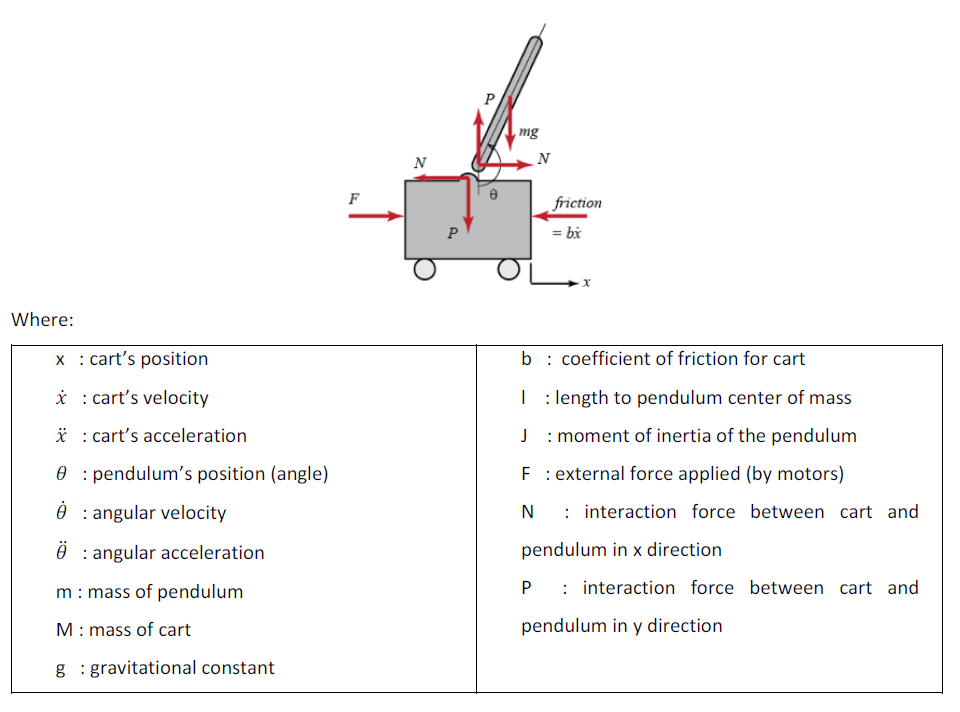
\includegraphics[width=0.7\textwidth]{figures/cart.png}
		\caption{graphical description of the model}
		\label{fig:scheme}
\end{figure}

The equations of the model are given by: 

	\begin{eqnarray}
		\ddot{x} &=& \frac{1}{M} \sum_{cart} F_x = \frac{1}{M} \left( F - N - b\dot{x}\right)  \\
		\ddot{\Theta} &=& \frac{1}{I} \sum_{pend} \tau = \frac{1}{I} \left( -Nlcos\Theta - Plsin\Theta \right)  \\
		N &=& m\left( \ddot{x} - l\dot{\Theta}^2 sin\Theta + l\ddot{\Theta}cos\Theta\right)  \\
		P &=& m\left( l\ddot{\Theta}^2cos\Theta + l\ddot{\Theta}sin \Theta\right) 
	\end{eqnarray}
\newpage	
\subsection{Implementation in simulink}
The non linear model can be implemented using the equations above, this was already done in a previous lectore in the third semester. The resulting model can be seen in Figure~\ref{fig:non_linear_continuous}.
\begin{figure}[H]
		\centering
		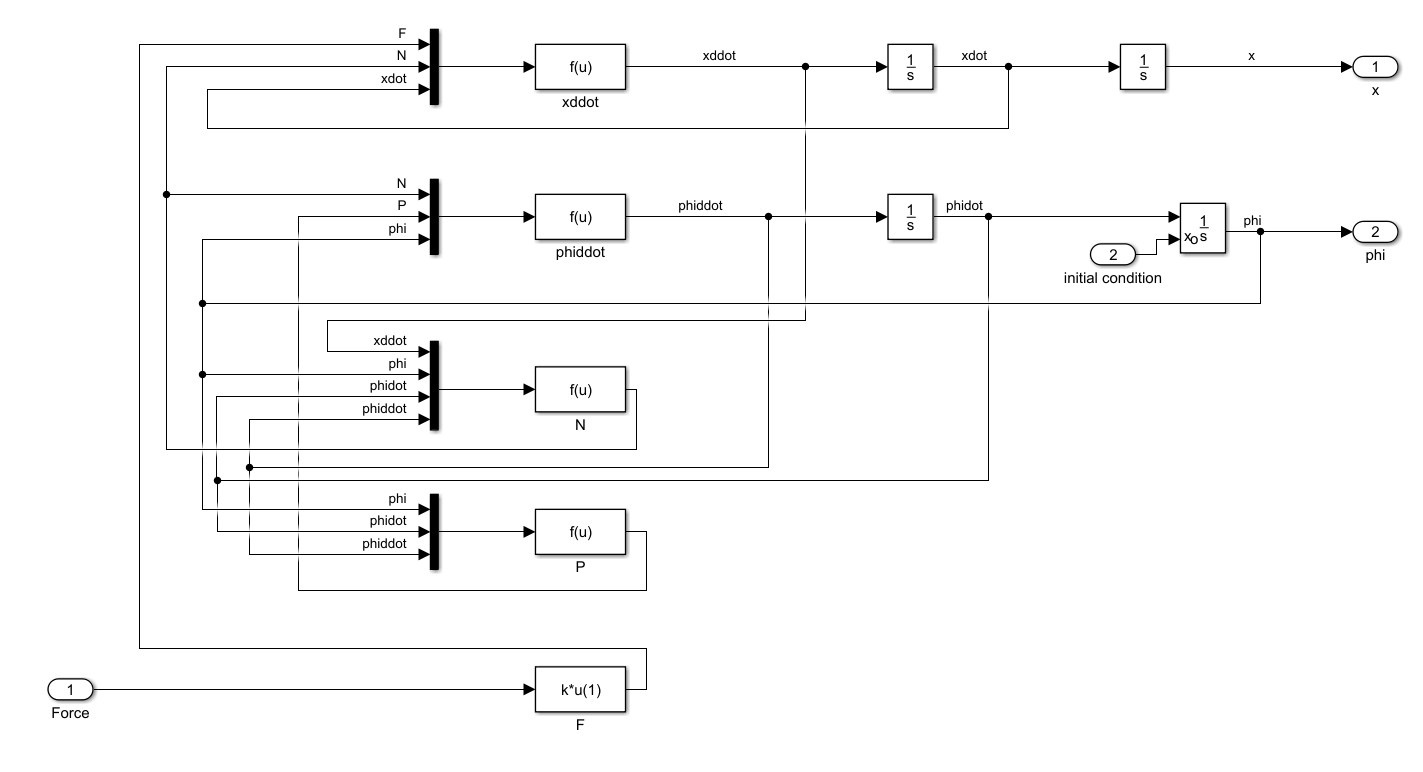
\includegraphics[width=0.7\textwidth]{figures/non_linear_continuous.png}
		\caption{Non linear continuous model in simulink}
		\label{fig:non_linear_continuous}
\end{figure}

\newpage
\section{Discretization from non-linear model}
Since the model will later be used on an actual hardware, it is important to sicretize the system. This is done by simply replacing the continuous time integrators with discrete time integrators. The settings of the integrators are shown in Figure~\ref{fig:integrator}.	
\begin{figure}[H]
		\centering
		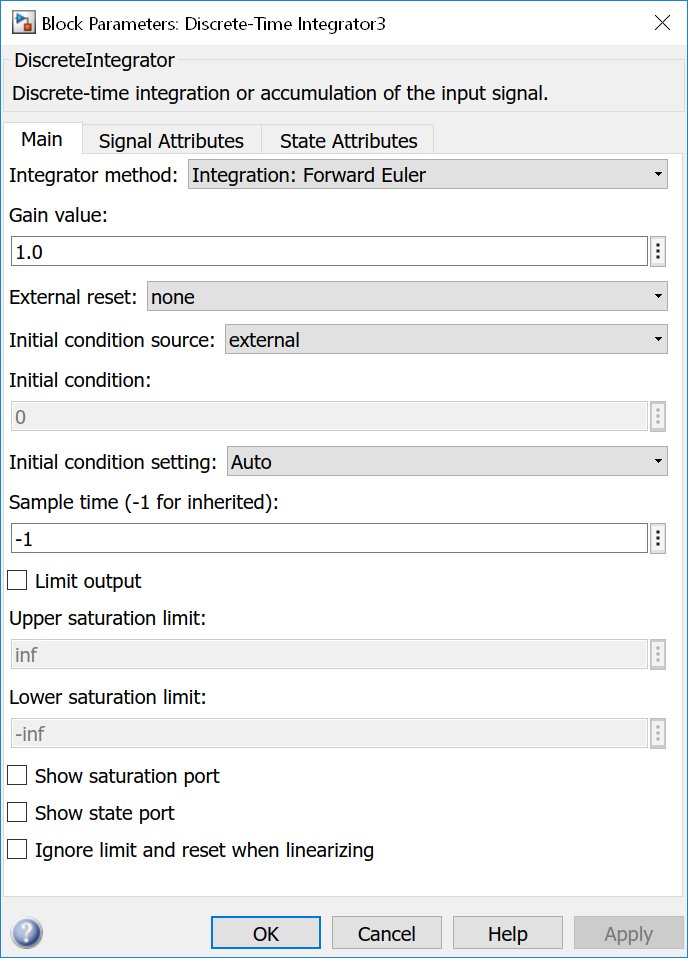
\includegraphics[width=0.7\textwidth]{figures/simulink_discrete_integrator.png}
		\caption{discrete time integrator settings}
		\label{fig:integrator}
\end{figure}	
\begin{figure}[H]
		\centering
		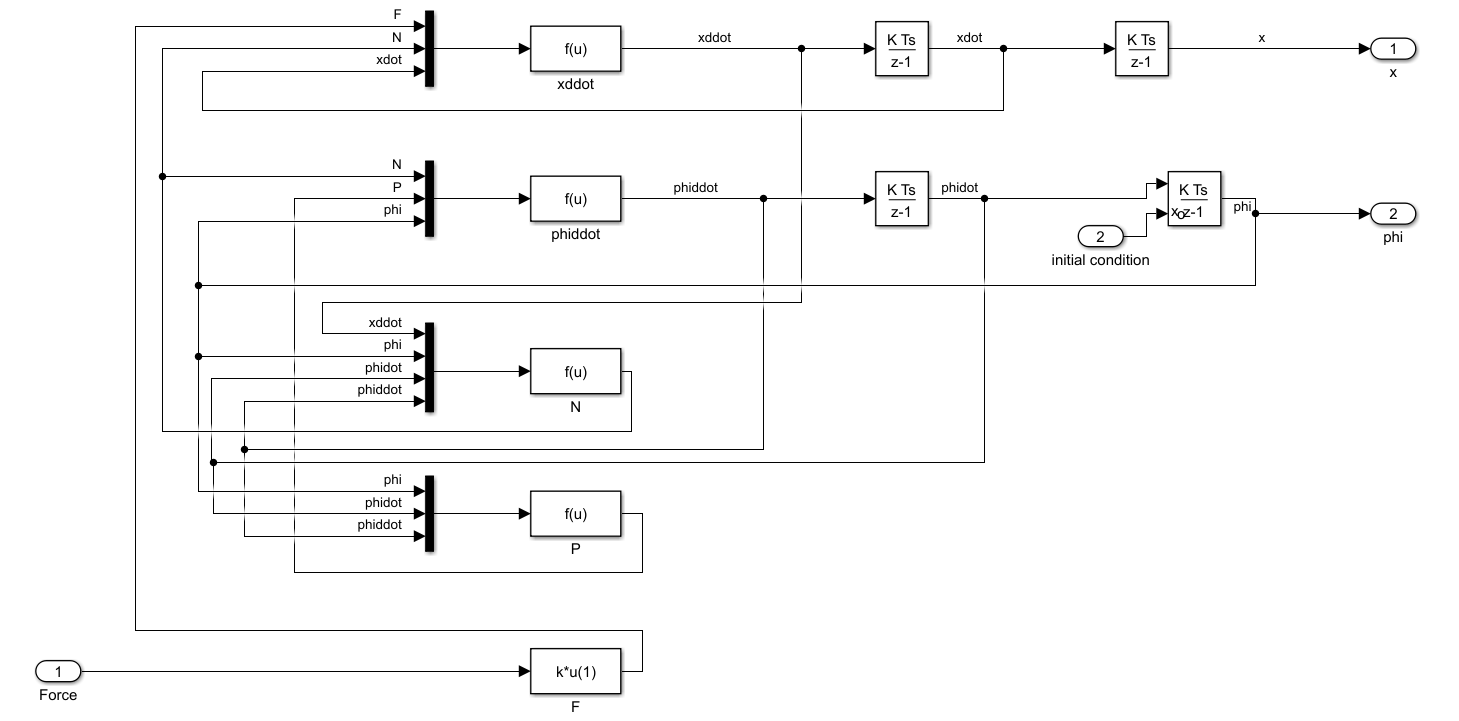
\includegraphics[width=0.7\textwidth]{figures/non_linear_discrete.png}
		\caption{Non linear discrete model in simulink}
		\label{fig:non_linear_continuous}
\end{figure}	

\subsection{Applying zero force to the system}
As a first test the model was tested with a constant of zero at its input. It would be expected to do nothing but stay upright since there are no external forces applied to the pendulum in the horizontal axis.	

\begin{figure}[H]
		\centering
		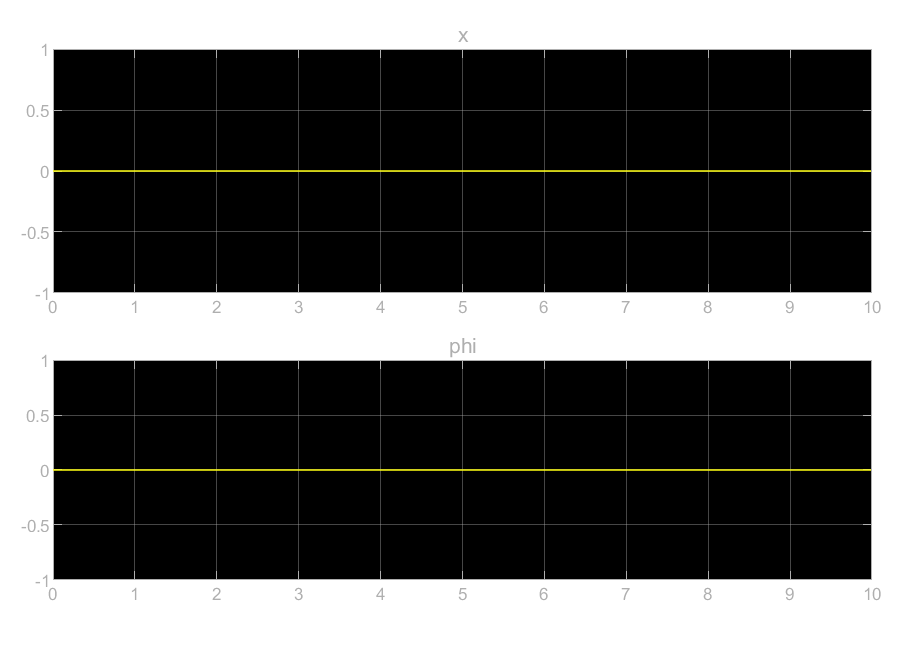
\includegraphics[width=0.7\textwidth]{figures/non_lin_disc_no_force.eps}
		\caption{Non linear discrete model simulation with zero force applied}
		\label{fig:non_linear_continuous}
\end{figure}
As a small test an initial step was applied to the system to see if it behaves correctly. The disturbance of the angle was accomplished by using the step function of simulink with an initial value of $10\cdot \frac{\pi}{180}$, which is 10° in radians.
As shown in Figure \ref{fig:sim_with_offset} the pendulum swings left and right and slowly loses height, so the model seems to be behaving correctly.
\begin{figure}[H]
		\centering
		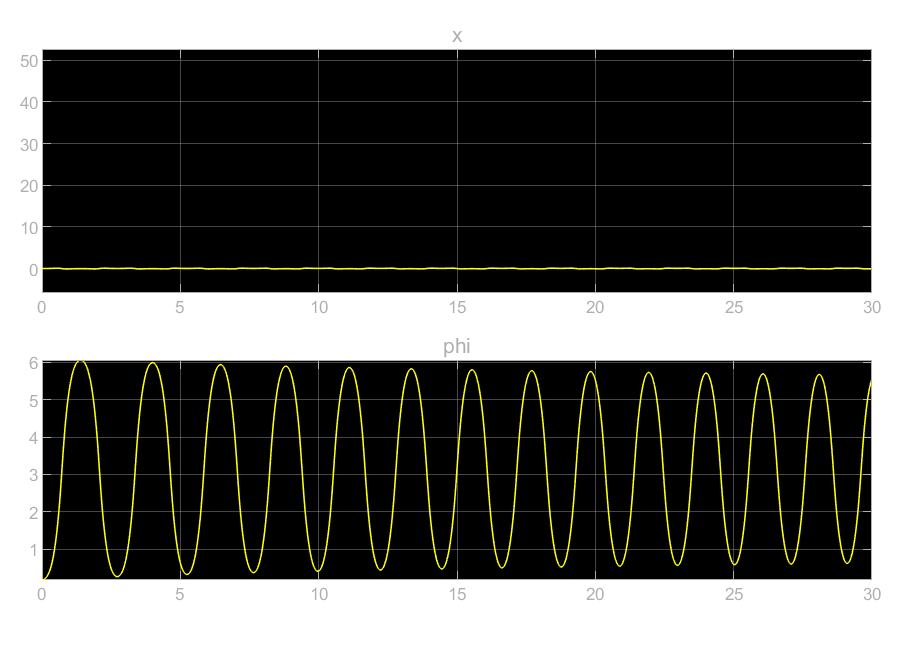
\includegraphics[width=0.7\textwidth]{figures/non_lin_disc_no_force_offset.eps}
		\caption{Non linear discrete model simulation with an offset step in the angle}
		\label{fig:sim_with_offset}
\end{figure}

\section{Linearization}
In order to further investigate the system for stability to make tuning the controller easier, it is mandatory to linearize the model. This is done by assuming that the slope of a sine wave is linear which of course is not the case but it is a valid approximation. The linearized equations are given by

	\begin{eqnarray}
		X\left(s\right)s^2&=&\frac{1}{M}\left(F\left(s\right)-mX\left(s\right)s^2+ml\Phi\left(s\right)s^2-bX\left(s\right)s\right)\\
		\Phi\left(s\right)s^2&=&\frac{1}{I}\ \left(mlX\left(s\right)s^2+mlg\Phi\left(s\right)-ml^2\Phi\left(s\right)s^2\right)
	\end{eqnarray}

From these equations the two transfer functions $G_1\left(s\right)=\frac{\Phi\left(s\right)}{F\left(s\right)}$ and $G_2\left(s\right)=\frac{X\left(s\right)}{F\left(s\right)}$ are to be found. This is simply a fact of rearranging the equations. \textbf{$G_1(s)$}
Solving equation 5 for $X(s)$:

\begin{eqnarray}
	X(s)\ s^2\ M&=&F(s)-mX(s)\ s^2+ml\Phi(s)\ s^2-bX(s)s \\
	X\left(s\right)s^2M&=&F\left(s\right)+ml\Phi\left(s\right)s^2+X\left(s\right)\left[-ms^2-bs\right] \\
	X\left(s\right)s^2M-X\left(s\right)\left[-ms^2-bs\right]&=&F\left(s\right)+ml\Phi\left(s\right)s^2 \\
	X\left(s\right)\left[s^2M+ms^2+bs\right]&=&F\left(s\right)+ml\Phi\left(s\right)s^2\\
	X\left(s\right)&=&\frac{F\left(s\right)+ml\Phi\left(s\right)s^2}{s^2M+ms^2+bs}
\end{eqnarray}

Inserting into equation 6 we get


\begin{eqnarray}
	\Phi\left(s\right)s^2=\frac{1}{I}\left[mls^2\cdot\frac{F\left(s\right)+ml\Phi\left(s\right)s^2}{s^2M+ms^2+bs}+mlg\Phi\left(s\right)-ml^2\Phi\left(s\right)s^2\right] \\
	\Phi\left(s\right)Is^2=mls^2\cdot\frac{F\left(s\right)+ml\Phi\left(s\right)s^2}{s^2M+ms^2+bs}+mlg\Phi\left(s\right)-ml^2\Phi\left(s\right)s^2 
	\\
	Is^2=mls^2\cdot\frac{\frac{F\left(s\right)}{\Phi\left(s\right)}+mls^2}{Ms^2+ms^2+bs}+mlg-ml^2s^2 \\
	Is^2=mls^2\cdot\frac{\frac{F\left(s\right)}{\Phi\left(s\right)}+mls^2}{Ms^2+ms^2+bs}+mlg-ml^2s^2 \\
	\frac{Is^2}{ml}=s^2\cdot\frac{\frac{F\left(s\right)}{\Phi\left(s\right)}+mls^2}{Ms^2+ms^2+bs}+g-ls^2 \\
	\frac{Is^2}{ml}=\frac{\frac{F\left(s\right)}{\Phi\left(s\right)}+mls^2}{M+m+\frac{b}{s}}+g-ls^2 \\
	\frac{F\left(s\right)}{\Phi\left(s\right)}=\left[\frac{I_s^2}{ml}-g+ls^2\right]\left[M+m+\frac{b}{s}\right]-mls^2 \\
	\frac{F\left(s\right)}{\Phi\left(s\right)}=\frac{MI}{ml}s^2+\frac{I}{l}s^2+\frac{Ib}{ml}s-gM-gm-\frac{gb}{s}+Mls^2+mls^2-mls^2 \\
	\frac{F\left(s\right)}{\Phi\left(s\right)}=s^2\left(\frac{MI}{ml}+\frac{I}{l}+Ml\right)+s\left(\frac{Ib}{ml}+lb\right)-gM-gm-\frac{gb}{s} \\
	\frac{\Phi\left(s\right)}{F\left(s\right)}=\frac{1}{s^2\left(\frac{MI}{ml}+\frac{I}{l}+Ml\right)+s\left(\frac{Ib}{ml}+lb\right)-gM-gm-\frac{gb}{s}} \\
	\frac{\Phi\left(s\right)}{F\left(s\right)}=\frac{s}{s^3\left(\frac{MI}{ml}+\frac{I}{l}+Ml\right)+s^2\left(\frac{Ib}{ml}+lb\right)+s(-gM-gm)-gb} 
	\\
	\frac{\Phi\left(s\right)}{F\left(s\right)}=\frac{s}{s^3\left(\frac{MI}{ml}+\frac{I}{l}+Ml\right)+s^2\left(\frac{Ib}{ml}+lb\right)+s\left(-gM-gm\right)-gb}
\end{eqnarray}


\textbf{$G_2(s)$}
Solving equation 6 for $\Phi(s)$:
\begin{eqnarray}
	\Phi\left(s\right)s^2=\frac{1}{I}\ \left(mlX\left(s\right)s^2+mlg\Phi\left(s\right)-ml^2\Phi\left(s\right)s^2\right)
	\\
	I\Phi\left(s\right)s^2=mlX\left(s\right)s^2+mlg\Phi\left(s\right)-ml^2\Phi\left(s\right)s^2
	\\
	\Phi\left(s\right)=\frac{mlX\left(s\right)s^2}{Is^2+ml^2s^2-mlg}
\end{eqnarray}

Inserting into the previously calculated transfer function:

\begin{eqnarray}
	\frac{\frac{mlX\left(s\right)s^2}{Is^2+ml^2s^2-mlg}}{F\left(s\right)}=\frac{s}{s^3\left(\frac{MI}{ml}+\frac{I}{l}+Ml\right)+s^2\left(\frac{Ib}{ml}+lb\right)+s(-gM-gm)-gb}
	\\
	\frac{X\left(s\right)}{F\left(s\right)}=\frac{Is^2+ml^2s^2-mlg}{mls^2}\cdot\frac{s}{s^3\left(\frac{MI}{ml}+\frac{I}{l}+Ml\right)+s^2\left(\frac{Ib}{ml}+lb\right)+s(-gM-gm)-gb}
	\\
	\frac{X\left(s\right)}{F\left(s\right)}=\frac{Is^2+ml^2s^2-mlg}{\ mls\cdot\left[s^3\left(\frac{MI}{ml}+\frac{I}{l}+Ml\right)+s^2\left(\frac{Ib}{ml}+lb\right)+s\left(-gM-gm\right)-gb\right]}
	\\
	\frac{X\left(s\right)}{F\left(s\right)}=\frac{s^2\left(I+ml^2\right)-mlg}{s^4\left(MI+Im+Mml^2\right)+s^3\left(Ib+m{bl}^2\right)+s^2\left(-gml\left[M+m\right]\right)-s\left(gbml\right)}
	\\
\end{eqnarray}

Our two transfer functions are therefore
\begin{eqnarray}
	G_1\left(s\right)=\frac{\Phi\left(s\right)}{F\left(s\right)}=\frac{s}{s^3\left(\frac{MI}{ml}+\frac{I}{l}+Ml\right)+s^2\left(\frac{Ib}{ml}+lb\right)+s(-gM-gm)-gb}
	\\
	G_2\left(s\right)=\frac{X\left(s\right)}{F\left(s\right)}=\frac{s^2\left(I+ml^2\right)-mlg}{s^4\left(MI+Im+Mml^2\right)+s^3\left(Ib+m{bl}^2\right)+s^2\left(-gml\left[M+m\right]\right)-s\left(gbml\right)}
\end{eqnarray}

To validate the calculations, the results were compared to the ones yielded in the online documentation\footnote{http://ctms.engin.umich.edu/CTMS/index.php?example=InvertedPendulum\&section=SystemModeling}.  The poles and zeros matched and therefore it can be assumed that the calculations are correct.

\section{Discretization linear model}

	\subsection{Forward Euler}
	
		\begin{eqnarray}
			z = e^{sT} \approx 1 + sT \rightarrow s \approx \frac{z - 1}{T}\\
			G_1\left(z\right) \approx \frac{\frac{z - 1}{T}}{\left( \frac{z - 1}{T}\right) ^3\left(\frac{MI}{ml}+\frac{I}{l}+Ml\right)+\left( \frac{z - 1}{T}\right) ^2\left(\frac{Ib}{ml}+lb\right)+\frac{z - 1}{T}(-gM-gm)-gb}\\
			G_2\left(z\right)=\frac{\left( \frac{z - 1}{T}\right) ^2\left(I+ml^2\right)-mlg}{\left( \frac{z - 1}{T}\right) ^4\left(MI+Im+Mml^2\right)+\left( \frac{z - 1}{T}\right) ^3\left(Ib+m{bl}^2\right)+\left( \frac{z - 1}{T}\right) ^2\left(-gml\left[M+m\right]\right)-\frac{z - 1}{T}\left(gbml\right)}
		\end{eqnarray}
	
	\subsection{Backward Euler}
		
		\begin{eqnarray}
			z = e^{sT} \approx \frac{1}{1 + sT} \rightarrow s \approx \frac{z - 1}{Tz}\\			
			G_1\left(z\right)=\frac{\frac{z - 1}{Tz}}{\left( \frac{z - 1}{Tz}\right) ^3\left(\frac{MI}{ml}+\frac{I}{l}+Ml\right)+\left( \frac{z - 1}{Tz}\right) ^2\left(\frac{Ib}{ml}+lb\right)+\frac{z - 1}{Tz}(-gM-gm)-gb}
			\\
			G_2\left(z\right)=\frac{\left( \frac{z - 1}{Tz}\right) ^2\left(I+ml^2\right)-mlg}{\left( \frac{z - 1}{Tz}\right) ^4\left(MI+Im+Mml^2\right)+s^3\left(Ib+m{bl}^2\right)+\left( \frac{z - 1}{Tz}\right) ^2\left(-gml\left[M+m\right]\right)-\frac{z - 1}{Tz}\left(gbml\right)}
		\end{eqnarray}
	
	\subsection{Trapezoidal or Tustin}
		\begin{tiny}
		\begin{eqnarray}
			z = e^{sT} \approx \frac{1 + sT/2}{1 - sT/2} \rightarrow s \approx \frac{2\left( z - 1\right) }{T\left( z+1\right) }\\		
			G_1\left(z\right)=\frac{\frac{2\left( z - 1\right) }{T\left( z+1\right) }}{\left( \frac{2\left( z - 1\right) }{T\left( z+1\right) }\right) ^3\left(\frac{MI}{ml}+\frac{I}{l}+Ml\right)+\left( \frac{2\left( z - 1\right) }{T\left( z+1\right) }\right) ^2\left(\frac{Ib}{ml}+lb\right)+\frac{2\left( z - 1\right) }{T\left( z+1\right) }(-gM-gm)-gb}
			\\
			G_2\left(z\right)=\frac{\left( \frac{2\left( z - 1\right) }{T\left( z+1\right) }\right) ^2\left(I+ml^2\right)-mlg}{\left( \frac{2\left( z - 1\right) }{T\left( z+1\right) }\right) ^4\left(MI+Im+Mml^2\right)+\left( \frac{2\left( z - 1\right) }{T\left( z+1\right) }\right) ^3\left(Ib+m{bl}^2\right)+\left( \frac{2\left( z - 1\right) }{T\left( z+1\right) }\right) ^2\left(-gml\left[M+m\right]\right)-\frac{2\left( z - 1\right) }{T\left( z+1\right) }\left(gbml\right)}
		\end{eqnarray}
		\end{tiny}
		
	\subsection{Discretizing using Matlab}
	Matlab has a built in function $c2d()$ that can discretize a continuous time transfer function. It only requires the transfer function and the sample time as an input. We using 0.0001 seconds as the sampling time. The Matlab code is shown below:
\begin{lstlisting}
cart_n2 = (I+m*l^2)/q;
cart_n1 = 0;
cart_n0 = -g*m*l/q;
cart_d4 = 1;
cart_d3 = b*(I+m*l^2)/q;
cart_d2 = ((M + m)*m*g*l)/q;
cart_d1 = - b*m*g*l/q;
cart_d0 = 0;

pend_n1 = m*l/q;
pend_n0 = 0;
pend_d3 = 1;
pend_d2 = (b*(I + m*l^2))/q;
pend_d1 = -((M + m)*m*g*l)/q;
pend_d0 = -b*m*g*l/q;

P_cart = (cart_n2*s^2 + cart_n1*s + cart_n0)/(cart_d4*s^4 + cart_d3*s^3 + cart_d2*s^2 + cart_d1*s + cart_d0)
P_pend = (pend_n1*s + pend_n0)/(pend_d3*s^3 + pend_d2*s^2 + pend_d1*s + pend_d0)


%% discretizing the transfer functions
d_P_cart = c2d(P_cart, 0.0001)
d_P_pend = c2d(P_pend, 0.0001)

\end{lstlisting}

This script puts out the discrete transfer function
\begin{equation}
	\frac{2.273\cdot 10^{-8}z^2-1.377\cdot 10^{-13} z-2.273\cdot 10^{-8}}{z^3-3z^2+3z-1}
\end{equation}
\todo{put in both equations}
\section{System analysis}
As a next step the transfer function of the systems shall be analysed using Matlab. This can be done using the command \textit{pzmap()}. 
\begin{lstlisting}
%Plotting poles and zeros 
figure
pzmap(P_cart, P_pend)
legend('cart','pendulum');

figure
pzmap(d_P_cart, d_P_pend)
legend('cart','pendulum');
\end{lstlisting}
This results in the following two figures.
\begin{figure}[H]
		\centering
		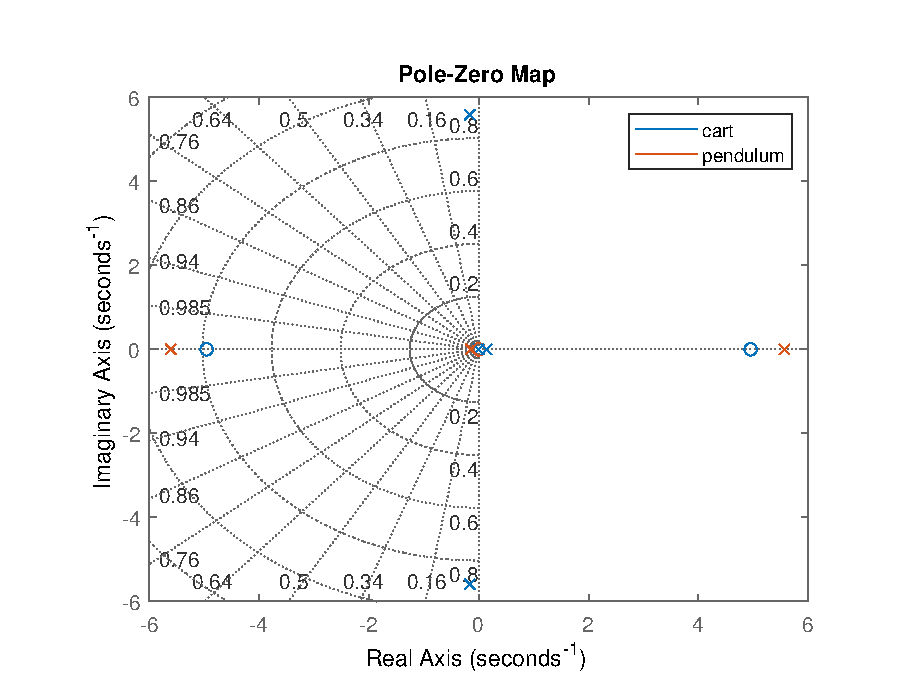
\includegraphics[width=0.7\textwidth]{figures/pzmap_cont.eps}
		\caption{pole and zero map of the continuous systems}
		\label{fig:pzmap_cont}
\end{figure}
\begin{figure}[H]
		\centering
		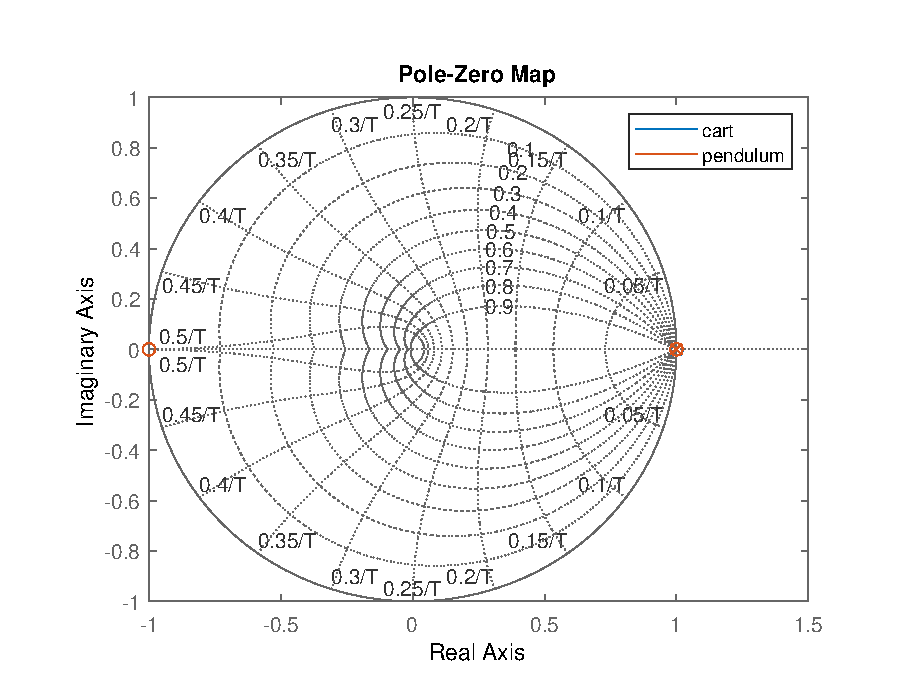
\includegraphics[width=0.7\textwidth]{figures/pzmap_disc.eps}
		\caption{pole and zero map of the discrete systems}
		\label{fig:pzmap_disc}
\end{figure}
As figure ~\ref{fig:pzmap_cont} and ~\ref{fig:pzmap_disc} show both the cart and the pendulum are unstable no matter if discretized or not. For the continuous system this can be detected because the poles do not all have a negative imaginary part. Looking at the discrete system at first glance it looks like all poles are within or at last at the unit circle. However after zooming in (see Figure ~\ref{fig:pzmap_disc_zoomed}) it appears that a pole is outside of the unit circle which results in an unstable system.
\begin{figure}[H]
		\centering
		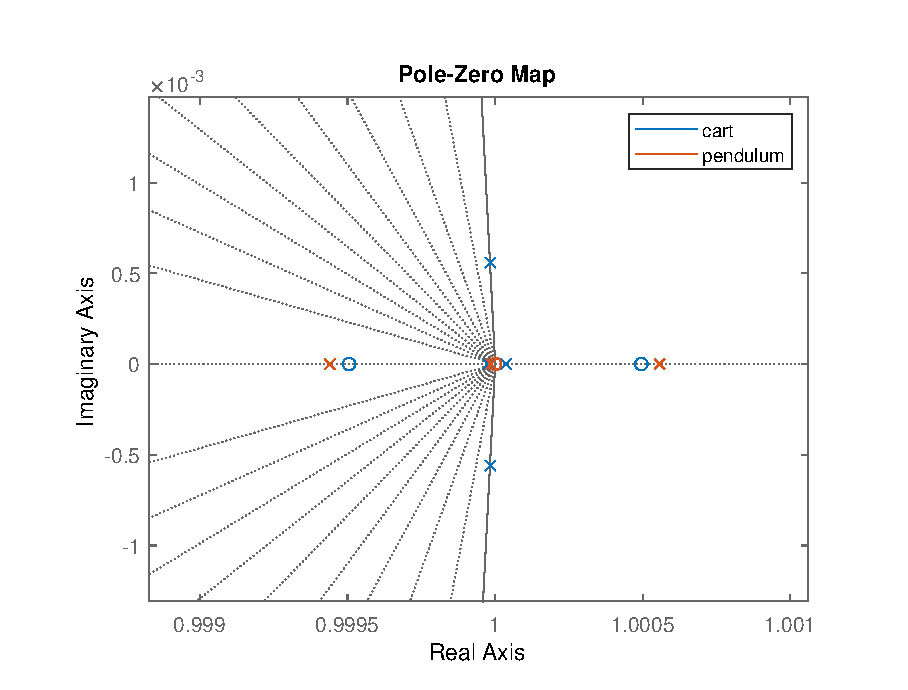
\includegraphics[width=0.7\textwidth]{figures/pzmap_disc_zoomed.eps}
		\caption{zoomed in pole and zero map of the discrete systems}
		\label{fig:pzmap_disc_zoomed}
\end{figure}
Next the both the discrete and the continuous model of the linearized model were implemented in simulink and tested next to each other. In order to get the denominator and the numerator of the transfer function for simulink, Matlabs \textit{tfdata} function was used.
\begin{figure}[H]
		\centering
		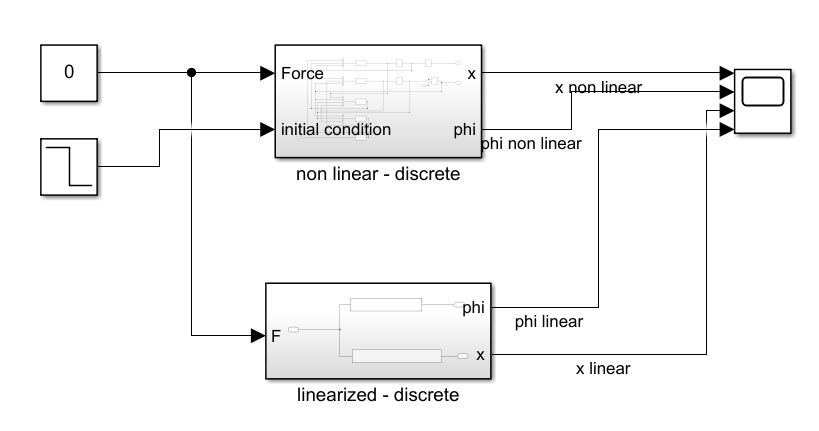
\includegraphics[width=0.7\textwidth]{figures/bothdiscrete_subsystems.png}
		\caption{linear and non linear version of the discrete system}
		\label{fig:both_discrete_subsystems}
\end{figure}
\begin{figure}[H]
		\centering
		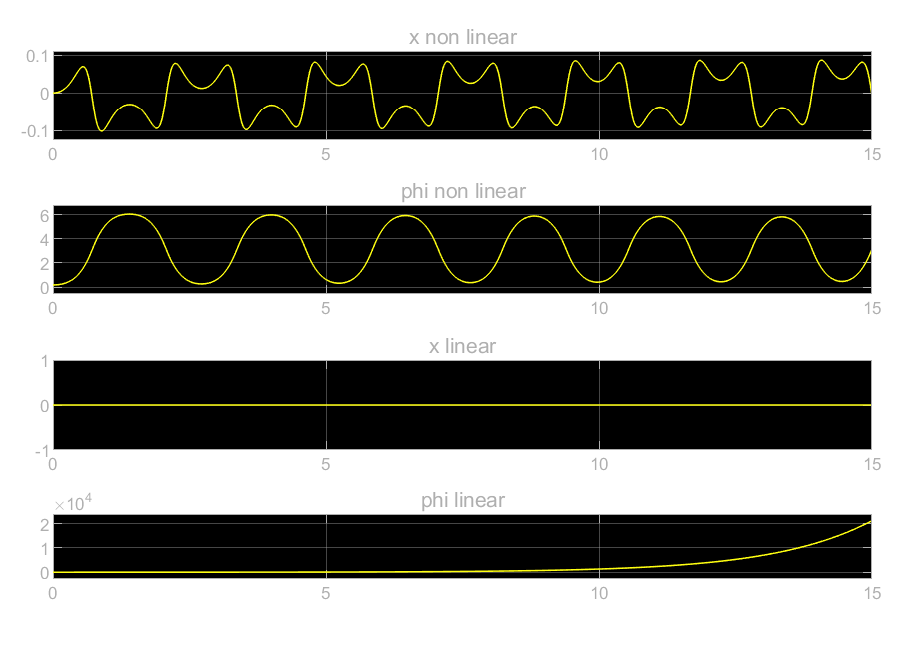
\includegraphics[width=0.7\textwidth]{figures/linear_vs_non_linear_discrete.eps}
		\caption{simulation result of linear and non linear version of the discrete system}
		\label{fig:both_discrete_subsystems_sim}
\end{figure}
As figure~\ref{fig:both_discrete_subsystems_sim} shows, the non linear system behaves the way it should. The pendulum starts swinging and slowly decreases in height. Due to the inertia of the system the cart moves a bit. At first sight the linearized model looks to be wonrg. However, this is not the case as it shows an exponential function which is the solution for the differential equation we're trying to solve. the linearized model only works with small deviations and small time slots, so in order for it to behave correctly we need to implement a controller that gets executed regularly.

\section{Control function}
Now that we have a working model of the pendulum we are going to have to control the cart in such a way, that it always keeps the pendulum upwards. For this purpose two models are going to be developed: one using the continuous plant and the other using the discrete one. The controller we'll be using is a simply PID controller that simulink offers. In addition a Kalman filter will be implemented in order to provide a more plausible vertical position coming form the plant.
Firstly, the provided Kalman filter was implemented using the Matlab function block and to test it the following model was built and simulated:
\begin{figure}[H]
		\centering
		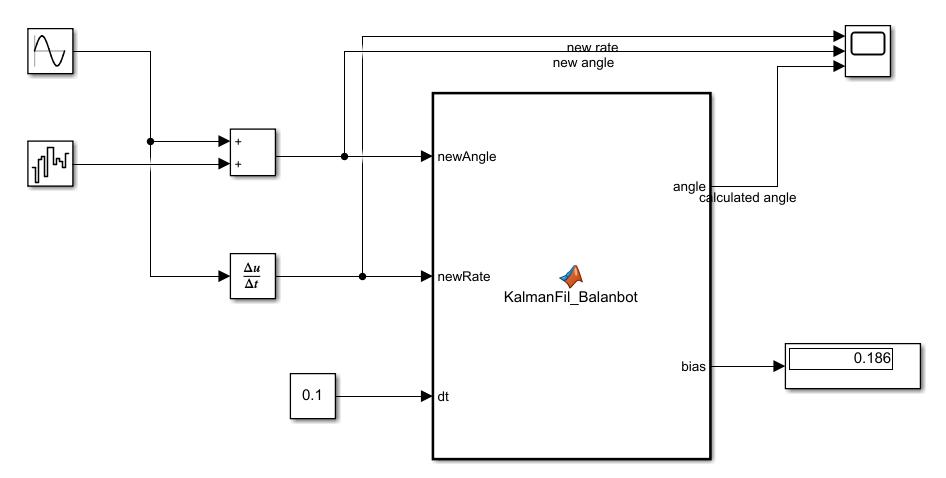
\includegraphics[width=0.7\textwidth]{figures/kalman_test.png}
		\caption{Kalman filter test model}
		\label{fig:kalman_test}
\end{figure}
\begin{figure}[H]
		\centering
		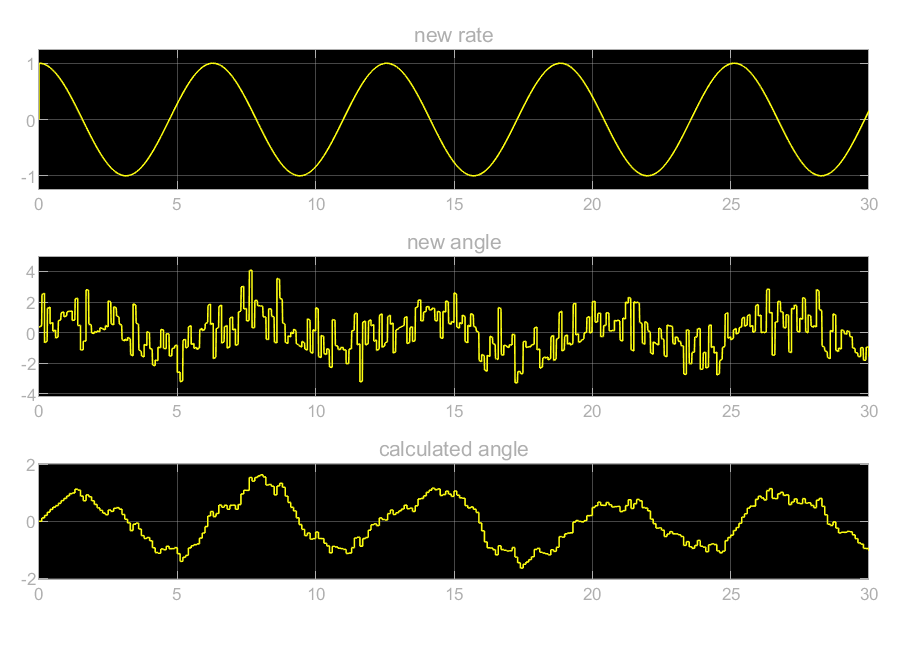
\includegraphics[width=0.7\textwidth]{figures/kalman_test_results.eps}
		\caption{Kalman filter test results}
		\label{fig:kalman_test_results}
\end{figure}
As Figure ~\ref{fig:kalman_test} shows, the filter works quite well, so we can move onto implementing the PID controllers. Now two simulink models were developed. One with the discrete plant and one with the continuous one. The controller was in both cases discrete. For simulation purposes the Kalman filter was implemented using the deviation o fthe angle in order to gain the angular velocity.
\begin{figure}[H]
		\centering
		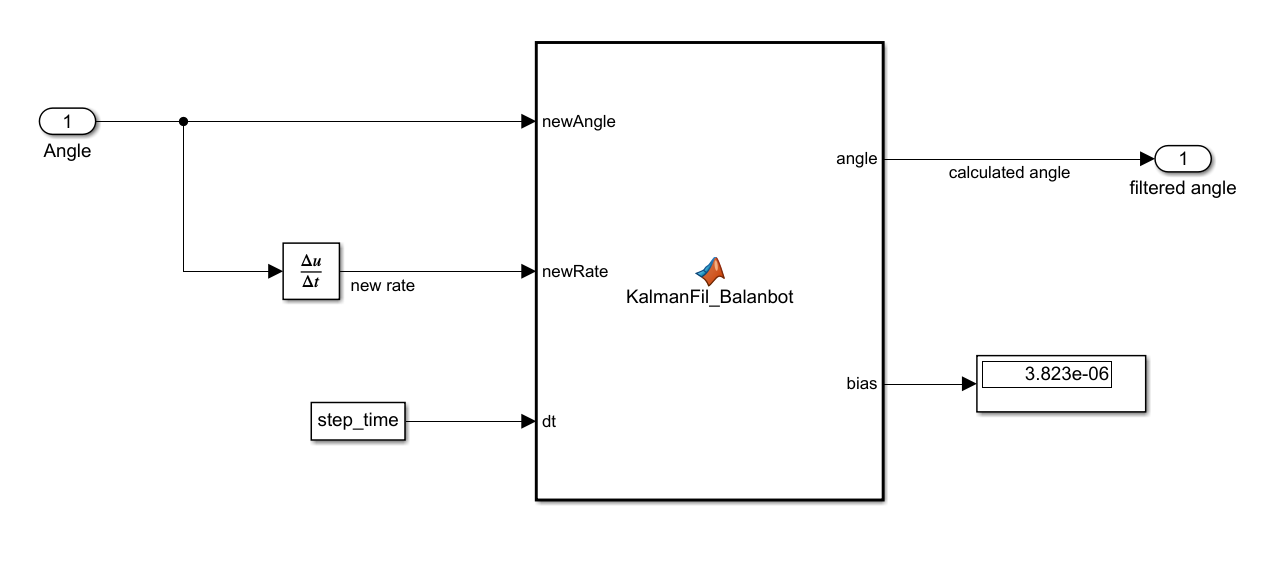
\includegraphics[width=0.7\textwidth]{figures/Kalman_sim.png}
		\caption{Kalman filter for simulation}
		\label{fig:kalman_sim}
\end{figure}
Now the continuous system was built and simulated using a variable step solver.
\begin{figure}[H]
		\centering
		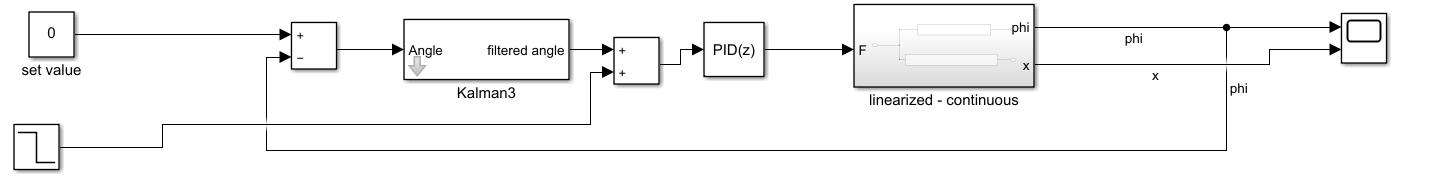
\includegraphics[width=0.7\textwidth]{figures/linear_balan_bot_cont.png}
		\caption{linearized continuous system simulation setup}
		\label{fig:lin_cont_sim}
\end{figure}
\begin{figure}[H]
		\centering
		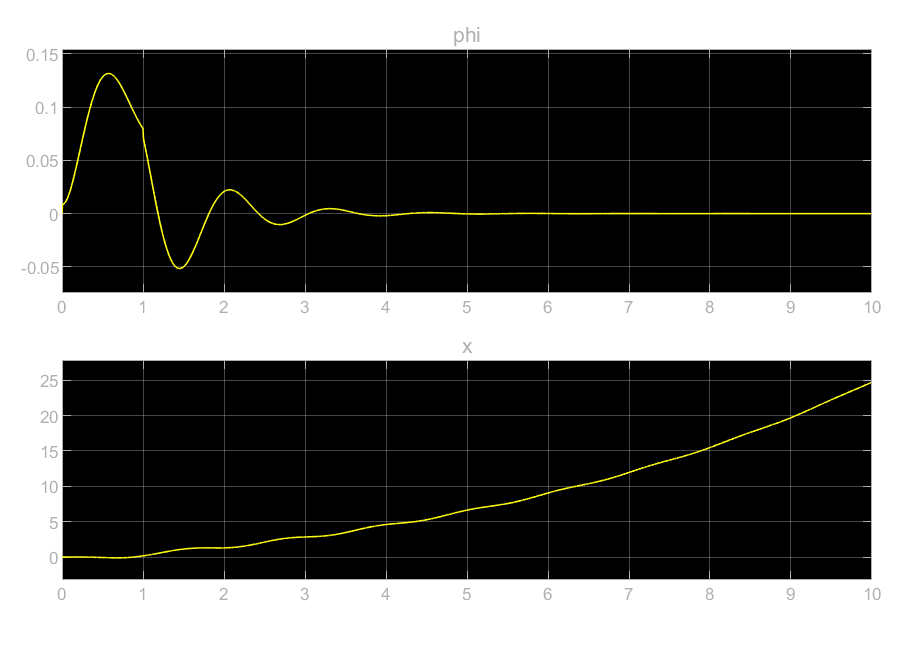
\includegraphics[width=0.7\textwidth]{figures/linear_balan_bot_cont_sim.eps}
		\caption{linearized continuous system simulation results}
		\label{fig:lin_cont_res}
\end{figure}
After that the same was done for the discrete system. This time a fixed step discrete solver was used.
\begin{figure}[H]
		\centering
		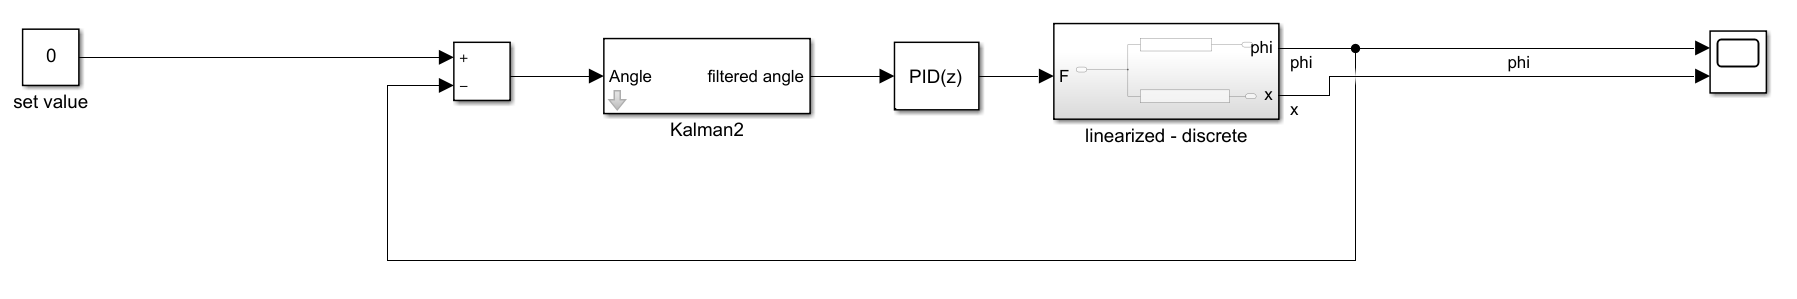
\includegraphics[width=0.7\textwidth]{figures/linear_balan_bot_disc.png}
		\caption{linearized discrete system simulation setup}
		\label{fig:lin_disc_sim}
\end{figure}
\begin{figure}[H]
		\centering
		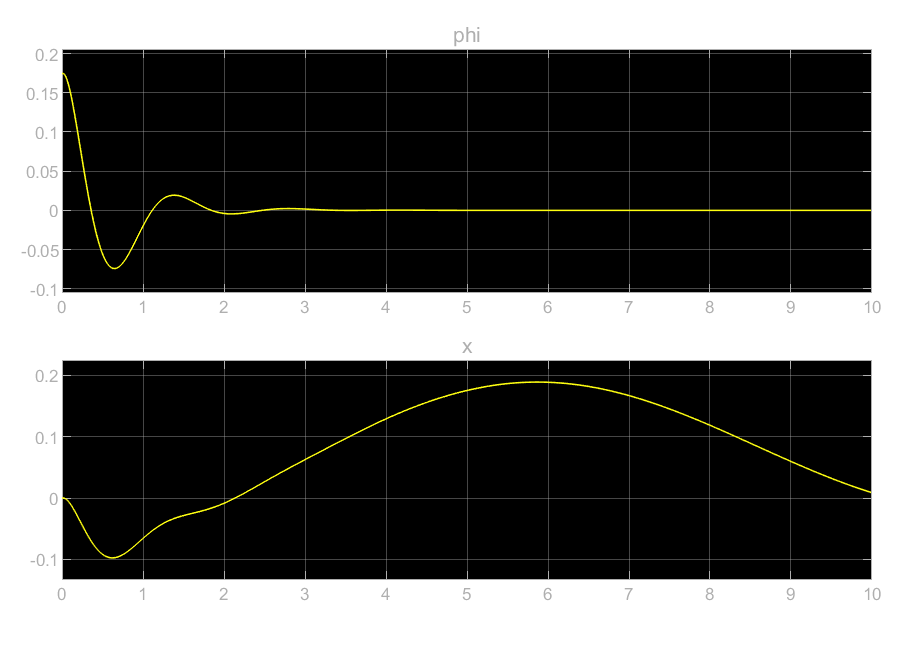
\includegraphics[width=0.7\textwidth]{figures/linear_balan_bot_disc_sim.eps}
		\caption{linearized discrete system simulation results}
		\label{fig:lin_disc_res}
\end{figure}

In both cases the models seem to behave the way they should, the controllers also seem to be working well so we can move on to the next step which is deploying the whole thing onto the actual hardware.





	
	\clearpage
\part{Laboratory Session 07}
\section{Introduction}
In this session everything was prepared to put the BalanBot into operation. For this purpose, a block was created for initialization. Another block reads the sensors. These evaluated sensor data are filtered and converted into wheel rotation with a PID controller.
Unfortunately all BalanBots were already borrowed when everything was ready on friday the first of february.

\section{System Initialization}
First the MPU6050 has to be initialized. This was done using $I^2C$ communication.
A value was assigned to the individual registers at the slave address 0x68.
For example, register 0x19 was assigned the value 7. So the sample rate was set with the formula:\\
	\begin{equation}
		1000Hz - \frac{8000Hz}{n-1}
	\end{equation}
In this formula n was replaced by seven.	\\
%\todo{Priority???}\\

	\begin{figure}[H]
		\centering
		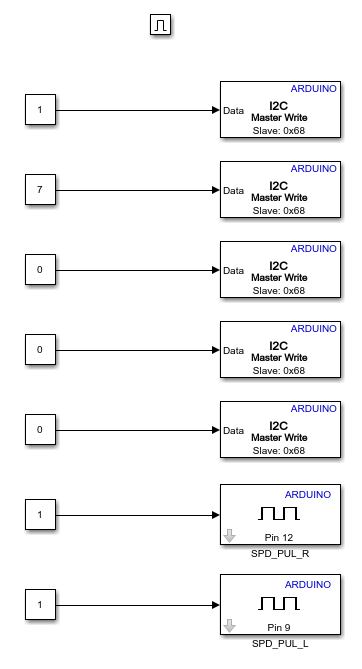
\includegraphics[width=0.275\textwidth]{figures/init.PNG}
		\caption{The initialization}	
		Source: Own presentation	
		\label{fig:init}	
	\end{figure}
%	\begin{mdframed}
%		\begin{lstlisting}[caption={C-Code from the script}, language=c,label={lst:init}]
%	i2cData[0] = 7; // Set the sample rate to 1000Hz - 8kHz/(7+1) = 1000Hz
%	i2cData[1] = 0x00; // Disable FSYNC and set 260 Hz Acc filtering, 256 Hz Gyro filtering, 8 KHz sampling
%	i2cData[2] = 0x00; // Set Gyro Full Scale Range to +-250deg/s
%	i2cData[3] = 0x00; // Set Accelerometer Full Scale Range to +-2g
%	while (i2cWrite(0x19, i2cData, 4, false)); // Write to all four registers at once
%	while (i2cWrite(0x6B, 0x01, true)); // PLL with X axis gyroscope reference and disable sleep mode		
%		\end{lstlisting}
%	\end{mdframed}	
%	\todo{Löschen?????}
%	\begin{mdframed}
%		\begin{lstlisting}[caption={Automatic generated C-Code from the model}, language=c,label={lst:init_real}]
%	/* Start for Enabled SubSystem: '<Root>/One_time_initialization' */
%	/* Constant: '<S1>/Constant1' */
%	framework_I2CWrite4_Start(&framework_DW.I2CWrite);
%	
%	/* Constant: '<S1>/Constant2' */
%	framework_I2CWrite4_Start(&framework_DW.I2CWrite1);
%	
%	/* Constant: '<S1>/Constant3' */
%	framework_I2CWrite4_Start(&framework_DW.I2CWrite2);
%	
%	/* Constant: '<S1>/Constant4' */
%	framework_I2CWrite4_Start(&framework_DW.I2CWrite3);
%	
%	/* Start for MATLABSystem: '<S1>/I2C Write4' incorporates:
%	*  Constant: '<S1>/Constant5'
%	*/
%	framework_I2CWrite4_Start(&framework_DW.I2CWrite4);
%	
%	/* Start for MATLABSystem: '<S6>/Digital Output' */
%	framework_DW.obj_g.matlabCodegenIsDeleted = true;
%	framework_DW.obj_g.isInitialized = 0;
%	framework_DW.obj_g.matlabCodegenIsDeleted = false;
%	framework_DW.objisempty_f = true;
%	framework_DW.obj_g.isSetupComplete = false;
%	framework_DW.obj_g.isInitialized = 1;
%	digitalIOSetup(12, true);
%	framework_DW.obj_g.isSetupComplete = true;
%	
%	/* Start for MATLABSystem: '<S5>/Digital Output' */
%	framework_DW.obj_lq.matlabCodegenIsDeleted = true;
%	framework_DW.obj_lq.isInitialized = 0;
%	framework_DW.obj_lq.matlabCodegenIsDeleted = false;
%	framework_DW.objisempty_e1 = true;
%	framework_DW.obj_lq.isSetupComplete = false;
%	framework_DW.obj_lq.isInitialized = 1;
%	digitalIOSetup(9, true);
%	framework_DW.obj_lq.isSetupComplete = true;
%	
%	/* End of Start for SubSystem: '<Root>/One_time_initialization' */	
%	
%	/* Terminate for Enabled SubSystem: '<Root>/One_time_initialization' */
%	framework_I2CWrite4_Term(&framework_DW.I2CWrite);
%	framework_I2CWrite4_Term(&framework_DW.I2CWrite1);
%	framework_I2CWrite4_Term(&framework_DW.I2CWrite2);
%	framework_I2CWrite4_Term(&framework_DW.I2CWrite3);
%	
%	/* Terminate for MATLABSystem: '<S1>/I2C Write4' */
%	framework_I2CWrite4_Term(&framework_DW.I2CWrite4);
%	
%	/* Terminate for MATLABSystem: '<S6>/Digital Output' */
%	matlabCodegenHandle_matlabCod_f(&framework_DW.obj_g);
%	
%	/* Terminate for MATLABSystem: '<S5>/Digital Output' */
%	matlabCodegenHandle_matlabCod_f(&framework_DW.obj_lq);
%	
%	/* End of Terminate for SubSystem: '<Root>/One_time_initialization' */		
%		\end{lstlisting}
%	\end{mdframed}

	
\section{Read Sensor Datas}\label{sec:read}
	\begin{figure}[!htbp]
		\centering
		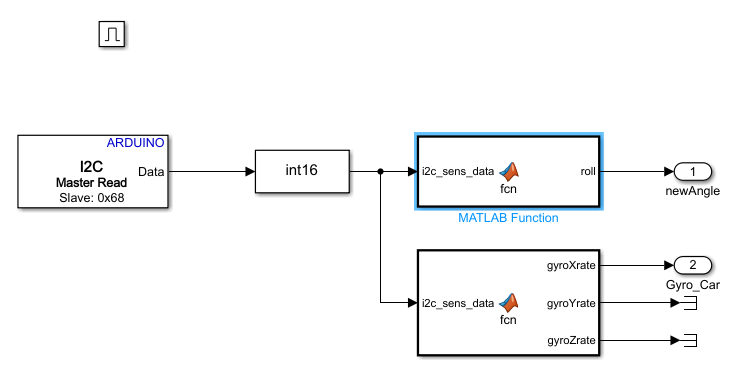
\includegraphics[width=0.7\textwidth]{figures/read.PNG}
		\caption{Processing of the read datas}	
		Source: Own presentation	
		\label{fig:read}	
	\end{figure}
The sensor data is processed in this block. First they are converted into the data type int16. 
Then the bus signal is splited into angle and gyro.
	\subsection{Angle}
	The Pythagorean theorem is used to calculate the absolute value of accX and accZ. With this value and accY the arctan finally calculates the angle in radians. At the end the angle is converted into degrees. Sown in Listing \ref{lst:roll}.
		\begin{mdframed}
			\begin{lstlisting}[caption={Conversion from the acceleration to the angle}, language=matlab,label={lst:roll}]
			function roll = fcn(i2c_sens_data)
			accX = double(i2c_sens_data(1));
			accY = double(i2c_sens_data(2));
			accZ = double(i2c_sens_data(3));
			roll = atan(accY / sqrt(accX * accX + accZ * accZ)) * 180/pi;		
			\end{lstlisting}
		\end{mdframed}
	
	\subsection{Gyro}
	The data from the gyro sensor is converted to double format and then divided by 131. Shown in Listing \ref{lst:gyro}.
%	\todo{why /131???}
		\begin{mdframed}
			\begin{lstlisting}[caption={Conversion to the gyros}, language=matlab,label={lst:gyro}]
			function [gyroXrate,gyroYrate,gyroZrate] = fcn(i2c_sens_data)
			gyroX = double(i2c_sens_data(5));
			gyroY = double(i2c_sens_data(6));
			gyroZ = double(i2c_sens_data(7));
			gyroXrate = gyroX/131;
			gyroYrate = gyroY/131;
			gyroZrate = gyroZ/131;	
			\end{lstlisting}
		\end{mdframed}
	
%	\subsection{Test in External Mode}
%	\todo{Was stellten wir fest}
%	

\section{Controller}
The controller now uses the sensor data prepared in Section \ref{sec:read}. First, measurement errors are reduced with the kalman filter.
Then the filtered angle is converted into a PWM signal by a PID controller.
For the factors of the PID controller the values recommended in the script were taken first. In external mode the PID parameters would have been finally adjusted. Due to the lack of hardware this could not be done. \\
%These were finally adjusted by tests on the BalanBot. For this purpose, the simulation in Simulink was run in the external mode.\\
\todo{Simulationsparameter erklären und beschreiben wieso si nicht stimmen können}

%\todo{replace figure with update values and descripe the new Values}
%
%	\subsection{Kp}
%	xx
%	\subsection{Ki}
%	xx
%	\subsection{Kd}
%	xx
	
	\begin{figure}[H]
		\centering
		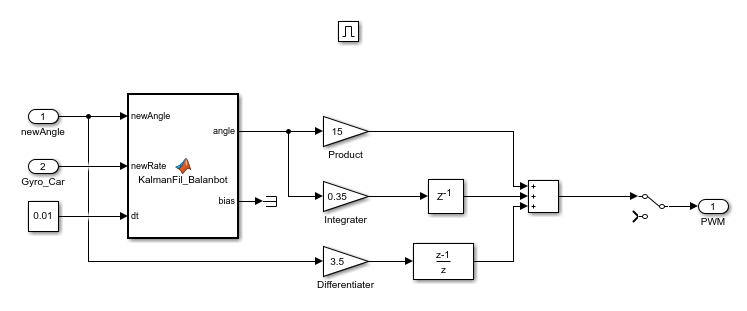
\includegraphics[width=0.7\textwidth]{figures/controller.PNG}
		\caption{Kalman Filter and PID Controller}	
		Source: Own presentation	
		\label{fig:controller}	
	\end{figure}


\section{Actuators}
The direction of rotation of the motors is done with an H-bridge of the digital outputs at pins 3, 4, 7 and 8. If the PWM input is greater than zero, the motors rotate in one direction. If it is smaller, they rotate in the other direction.
This PWM input value is finally converted into a PWM signal.\\
If the input is zero, the signal is constant zero. The larger this input is, the wider the PWM signal becomes. If this value is greater than or equal to 255, the signal is constant 1. This conversion is done with the blocks assigned to ports 5 and 6.

	\begin{figure}[H]
		\centering
		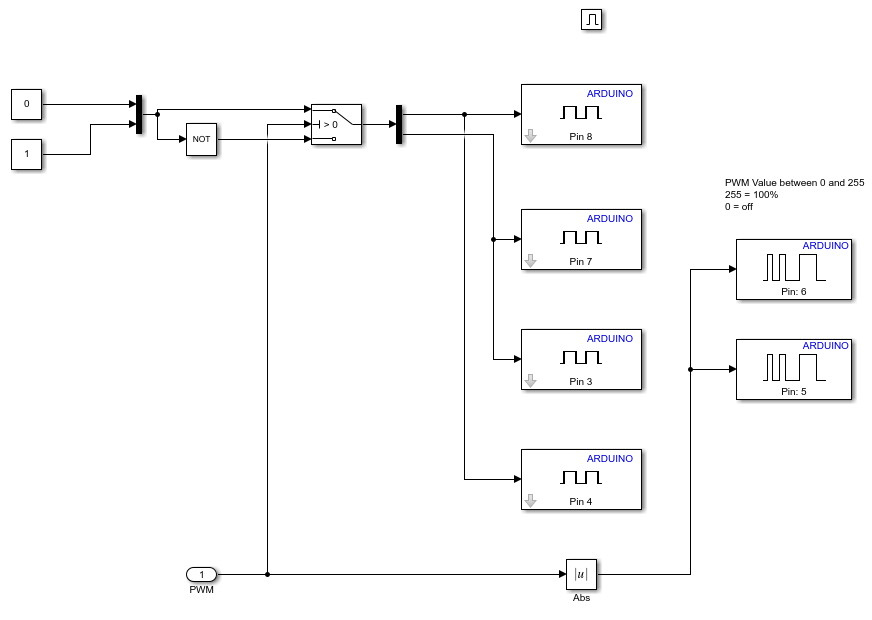
\includegraphics[width=0.7\textwidth]{figures/act.PNG}
		\caption{Converts the PWM input in direction of rotation and speedo}	
		Source: Own presentation	
		\label{fig:act}	
	\end{figure}


\section{Whole Structure}
Finally, all the blocks from the previous sections were assembled to form a single structure shown in Figure \ref{fig:struct}.

	\begin{figure}[!htbp]
		\centering
		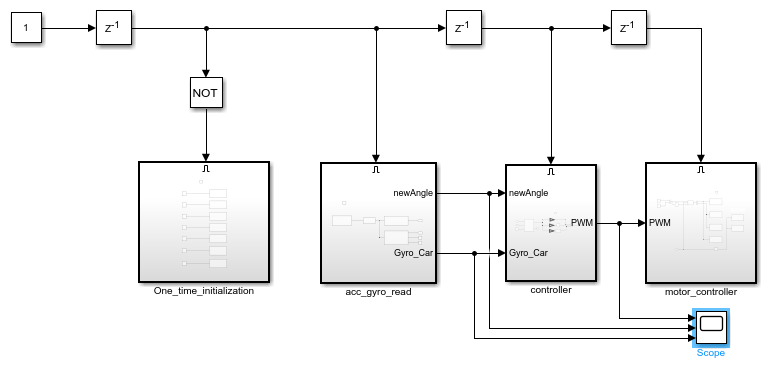
\includegraphics[width=0.7\textwidth]{figures/struct.PNG}
		\caption{The whole structure consist of blocks from the previous sections}	
		Source: Own presentation	
		\label{fig:struct}	
	\end{figure}

%\section{Test with the BalanBot}
%When simulating in external mode the PID controller could be adjusted. The cable did not turn out to be advantageous.
%The adjustment of the PID values required a lot of patience and know-how.

\section{Conclusion}
Everything was prepared to load the automatically generated code onto the BalanBot and to adjust the PID parameters and to perform further tests and analyses. Unfortunately all BalanBots were borrowed three days before the delivery.\\
A part of the automatically generated C code can be found in the appendix.


\cleardoublepage
\appendix
\section{Appendix}

%	\begin{mdframed}
		\begin{lstlisting}[caption={Automatically generated C code}, language=c,label={lst:acg}]
/*
* framework.c
*
* Academic License - for use in teaching, academic research, and meeting
* course requirements at degree granting institutions only.  Not for
* government, commercial, or other organizational use.
*
* Code generation for model "framework".
*
* Model version              : 1.7
* Simulink Coder version : 9.0 (R2018b) 24-May-2018
* C source code generated on : Fri Feb  1 19:59:15 2019
*
* Target selection: grt.tlc
* Note: GRT includes extra infrastructure and instrumentation for prototyping
* Embedded hardware selection: Intel->x86-64 (Windows64)
* Code generation objectives: Unspecified
* Validation result: Not run
*/

#include "framework.h"
#include "framework_private.h"

/* Block signals (default storage) */
B_framework_T framework_B;

/* Block states (default storage) */
DW_framework_T framework_DW;

/* Real-time model */
RT_MODEL_framework_T framework_M_;
RT_MODEL_framework_T *const framework_M = &framework_M_;

/* Forward declaration for local functions */
static codertarget_arduinobase_int_e_T *arduinoI2CWrite_arduinoI2CWrite
(codertarget_arduinobase_int_e_T *obj);
static void framework_SystemCore_release(const codertarget_arduinobase_int_e_T
*obj);
static void framework_SystemCore_delete(const codertarget_arduinobase_int_e_T
*obj);
static void matlabCodegenHandle_matlabCodeg(codertarget_arduinobase_int_e_T *obj);

/* Forward declaration for local functions */
static codertarget_arduinobase_int_f_T *f_arduinoI2CRead_arduinoI2CRead
(codertarget_arduinobase_int_f_T *obj);
static codertarget_arduinobase_in_fe_T *arduino_PWMOutput_arduino_PWMOu
(codertarget_arduinobase_in_fe_T *obj);
static void matlabCodegenHandle_matlabCod_f(codertarget_arduinobase_block_T *obj);
static void framework_SystemCore_release_f(const codertarget_arduinobase_int_f_T
*obj);
static void framework_SystemCore_delete_fex(const
codertarget_arduinobase_int_f_T *obj);
static void matlabCodegenHandle_matlabC_fex(codertarget_arduinobase_int_f_T *obj);
static void matlabCodegenHandle_matlab_fex2(codertarget_arduinobase_in_fe_T *obj);
static codertarget_arduinobase_int_e_T *arduinoI2CWrite_arduinoI2CWrite
(codertarget_arduinobase_int_e_T *obj)
{
	codertarget_arduinobase_int_e_T *b_obj;
	obj->isInitialized = 0;
	b_obj = obj;
	obj->Hw.AvailablePwmPinNames.f1 = '2';
	obj->Hw.AvailablePwmPinNames.f2 = '3';
	obj->Hw.AvailablePwmPinNames.f3 = '4';
	obj->Hw.AvailablePwmPinNames.f4 = '5';
	obj->Hw.AvailablePwmPinNames.f5 = '6';
	obj->Hw.AvailablePwmPinNames.f6 = '7';
	obj->Hw.AvailablePwmPinNames.f7 = '8';
	obj->Hw.AvailablePwmPinNames.f8 = '9';
	obj->Hw.AvailablePwmPinNames.f9[0] = '1';
	obj->Hw.AvailablePwmPinNames.f9[1] = '0';
	obj->Hw.AvailablePwmPinNames.f10[0] = '1';
	obj->Hw.AvailablePwmPinNames.f10[1] = '1';
	obj->Hw.AvailablePwmPinNames.f11[0] = '1';
	obj->Hw.AvailablePwmPinNames.f11[1] = '2';
	obj->Hw.AvailablePwmPinNames.f12[0] = '1';
	obj->Hw.AvailablePwmPinNames.f12[1] = '3';
	obj->matlabCodegenIsDeleted = false;
	return b_obj;
}

static void framework_SystemCore_release(const codertarget_arduinobase_int_e_T
*obj)
{
	if ((obj->isInitialized == 1) && obj->isSetupComplete) {
		MW_I2C_Close(obj->MW_I2C_HANDLE);
	}
}

static void framework_SystemCore_delete(const codertarget_arduinobase_int_e_T
*obj)
{
	framework_SystemCore_release(obj);
}

static void matlabCodegenHandle_matlabCodeg(codertarget_arduinobase_int_e_T *obj)
{
	if (!obj->matlabCodegenIsDeleted) {
		obj->matlabCodegenIsDeleted = true;
		framework_SystemCore_delete(obj);
	}
}

/*
* Start for atomic system:
*    synthesized block
*    synthesized block
*    synthesized block
*    synthesized block
*    synthesized block
*/
void framework_I2CWrite4_Start(DW_I2CWrite4_framework_T *localDW)
{
	codertarget_arduinobase_int_e_T *obj;
	uint32_T i2cname;
	
	/* Start for MATLABSystem: '<S1>/I2C Write4' */
	localDW->obj.matlabCodegenIsDeleted = true;
	arduinoI2CWrite_arduinoI2CWrite(&localDW->obj);
	localDW->objisempty = true;
	obj = &localDW->obj;
	localDW->obj.isSetupComplete = false;
	localDW->obj.isInitialized = 1;
	i2cname = 0;
	obj->MW_I2C_HANDLE = MW_I2C_Open(i2cname, 0);
	localDW->obj.BusSpeed = 100000U;
	MW_I2C_SetBusSpeed(localDW->obj.MW_I2C_HANDLE, localDW->obj.BusSpeed);
	localDW->obj.isSetupComplete = true;
}

/*
* Output and update for atomic system:
*    synthesized block
*    synthesized block
*    synthesized block
*    synthesized block
*    synthesized block
*/
void framework_I2CWrite4(real_T rtu_0, DW_I2CWrite4_framework_T *localDW)
{
	uint8_T SwappedDataBytes[8];
	uint8_T b_SwappedDataBytes[9];
	real_T b_x;
	uint8_T xtmp;
	int32_T i;
	
	/* MATLABSystem: '<S1>/I2C Write4' */
	memcpy((void *)&SwappedDataBytes[0], (void *)&rtu_0, (uint32_T)((size_t)8 *
	sizeof(uint8_T)));
	xtmp = SwappedDataBytes[0];
	SwappedDataBytes[0] = SwappedDataBytes[7];
	SwappedDataBytes[7] = xtmp;
	xtmp = SwappedDataBytes[1];
	SwappedDataBytes[1] = SwappedDataBytes[6];
	SwappedDataBytes[6] = xtmp;
	xtmp = SwappedDataBytes[2];
	SwappedDataBytes[2] = SwappedDataBytes[5];
	SwappedDataBytes[5] = xtmp;
	xtmp = SwappedDataBytes[3];
	SwappedDataBytes[3] = SwappedDataBytes[4];
	SwappedDataBytes[4] = xtmp;
	memcpy((void *)&b_x, (void *)&SwappedDataBytes[0], (uint32_T)((size_t)1 *
	sizeof(real_T)));
	memcpy((void *)&SwappedDataBytes[0], (void *)&b_x, (uint32_T)((size_t)8 *
	sizeof(uint8_T)));
	b_SwappedDataBytes[0] = 107U;
	for (i = 0; i < 8; i++) {
		b_SwappedDataBytes[i + 1] = SwappedDataBytes[i];
	}
	
	MW_I2C_MasterWrite(localDW->obj.MW_I2C_HANDLE, 104U, b_SwappedDataBytes, 9U,
	false, false);
	
	/* End of MATLABSystem: '<S1>/I2C Write4' */
}

/*
* Termination for atomic system:
*    synthesized block
*    synthesized block
*    synthesized block
*    synthesized block
*    synthesized block
*/
void framework_I2CWrite4_Term(DW_I2CWrite4_framework_T *localDW)
{
	/* Terminate for MATLABSystem: '<S1>/I2C Write4' */
	matlabCodegenHandle_matlabCodeg(&localDW->obj);
}

static codertarget_arduinobase_int_f_T *f_arduinoI2CRead_arduinoI2CRead
(codertarget_arduinobase_int_f_T *obj)
{
	codertarget_arduinobase_int_f_T *b_obj;
	obj->isInitialized = 0;
	b_obj = obj;
	obj->Hw.AvailablePwmPinNames.f1 = '2';
	obj->Hw.AvailablePwmPinNames.f2 = '3';
	obj->Hw.AvailablePwmPinNames.f3 = '4';
	obj->Hw.AvailablePwmPinNames.f4 = '5';
	obj->Hw.AvailablePwmPinNames.f5 = '6';
	obj->Hw.AvailablePwmPinNames.f6 = '7';
	obj->Hw.AvailablePwmPinNames.f7 = '8';
	obj->Hw.AvailablePwmPinNames.f8 = '9';
	obj->Hw.AvailablePwmPinNames.f9[0] = '1';
	obj->Hw.AvailablePwmPinNames.f9[1] = '0';
	obj->Hw.AvailablePwmPinNames.f10[0] = '1';
	obj->Hw.AvailablePwmPinNames.f10[1] = '1';
	obj->Hw.AvailablePwmPinNames.f11[0] = '1';
	obj->Hw.AvailablePwmPinNames.f11[1] = '2';
	obj->Hw.AvailablePwmPinNames.f12[0] = '1';
	obj->Hw.AvailablePwmPinNames.f12[1] = '3';
	obj->matlabCodegenIsDeleted = false;
	return b_obj;
}

static codertarget_arduinobase_in_fe_T *arduino_PWMOutput_arduino_PWMOu
(codertarget_arduinobase_in_fe_T *obj)
{
	codertarget_arduinobase_in_fe_T *b_obj;
	obj->isInitialized = 0;
	b_obj = obj;
	obj->Hw.AvailablePwmPinNames.f1 = '2';
	obj->Hw.AvailablePwmPinNames.f2 = '3';
	obj->Hw.AvailablePwmPinNames.f3 = '4';
	obj->Hw.AvailablePwmPinNames.f4 = '5';
	obj->Hw.AvailablePwmPinNames.f5 = '6';
	obj->Hw.AvailablePwmPinNames.f6 = '7';
	obj->Hw.AvailablePwmPinNames.f7 = '8';
	obj->Hw.AvailablePwmPinNames.f8 = '9';
	obj->Hw.AvailablePwmPinNames.f9[0] = '1';
	obj->Hw.AvailablePwmPinNames.f9[1] = '0';
	obj->Hw.AvailablePwmPinNames.f10[0] = '1';
	obj->Hw.AvailablePwmPinNames.f10[1] = '1';
	obj->Hw.AvailablePwmPinNames.f11[0] = '1';
	obj->Hw.AvailablePwmPinNames.f11[1] = '2';
	obj->Hw.AvailablePwmPinNames.f12[0] = '1';
	obj->Hw.AvailablePwmPinNames.f12[1] = '3';
	obj->matlabCodegenIsDeleted = false;
	return b_obj;
}

static void matlabCodegenHandle_matlabCod_f(codertarget_arduinobase_block_T *obj)
{
	if (!obj->matlabCodegenIsDeleted) {
		obj->matlabCodegenIsDeleted = true;
	}
}

static void framework_SystemCore_release_f(const codertarget_arduinobase_int_f_T
*obj)
{
	if ((obj->isInitialized == 1) && obj->isSetupComplete) {
		MW_I2C_Close(obj->MW_I2C_HANDLE);
	}
}

static void framework_SystemCore_delete_fex(const
codertarget_arduinobase_int_f_T *obj)
{
	framework_SystemCore_release_f(obj);
}

static void matlabCodegenHandle_matlabC_fex(codertarget_arduinobase_int_f_T *obj)
{
	if (!obj->matlabCodegenIsDeleted) {
		obj->matlabCodegenIsDeleted = true;
		framework_SystemCore_delete_fex(obj);
	}
}

static void matlabCodegenHandle_matlab_fex2(codertarget_arduinobase_in_fe_T *obj)
{
	if (!obj->matlabCodegenIsDeleted) {
		obj->matlabCodegenIsDeleted = true;
	}
}

/* Model step function */
void framework_step(void)
{
	real_T F[4];
	real_T y;
	real_T K[2];
	static const real_T a[4] = { 0.001, 0.0, 0.0, 0.003 };
	
	int16_T b_output[7];
	uint8_T status;
	uint8_T output_raw[14];
	uint8_T y_0[2];
	int16_T x;
	uint8_T b_x[2];
	real_T rtb_Delay1;
	real_T rtb_Delay;
	int32_T i;
	real_T F_0[2];
	real_T tmp[2];
	real_T F_1[4];
	real_T F_2[4];
	real_T K_0;
	real_T P_tmp;
	
	/* Delay: '<Root>/Delay' */
	rtb_Delay = framework_DW.Delay_DSTATE;
	
	/* Outputs for Enabled SubSystem: '<Root>/One_time_initialization' incorporates:
	*  EnablePort: '<S1>/Enable'
	*/
	/* Logic: '<Root>/Logical Operator' incorporates:
	*  Constant: '<S1>/Constant1'
	*  Constant: '<S1>/Constant2'
	*  Constant: '<S1>/Constant3'
	*  Constant: '<S1>/Constant4'
	*  Delay: '<Root>/Delay'
	*/
	if (!(framework_DW.Delay_DSTATE != 0.0)) {
		framework_I2CWrite4(framework_P.Constant1_Value, &framework_DW.I2CWrite);
		framework_I2CWrite4(framework_P.Constant2_Value, &framework_DW.I2CWrite1);
		framework_I2CWrite4(framework_P.Constant3_Value, &framework_DW.I2CWrite2);
		framework_I2CWrite4(framework_P.Constant4_Value, &framework_DW.I2CWrite3);
		
		/* MATLABSystem: '<S1>/I2C Write4' incorporates:
		*  Constant: '<S1>/Constant1'
		*  Constant: '<S1>/Constant2'
		*  Constant: '<S1>/Constant3'
		*  Constant: '<S1>/Constant4'
		*  Constant: '<S1>/Constant5'
		*/
		framework_I2CWrite4(framework_P.Constant5_Value, &framework_DW.I2CWrite4);
		
		/* DataTypeConversion: '<S6>/Data Type Conversion' incorporates:
		*  Constant: '<S1>/Constant6'
		*/
		if (framework_P.Constant6_Value < 256.0) {
			if (framework_P.Constant6_Value >= 0.0) {
				status = (uint8_T)framework_P.Constant6_Value;
			} else {
				status = 0U;
			}
		} else {
			status = MAX_uint8_T;
		}
		
		/* End of DataTypeConversion: '<S6>/Data Type Conversion' */
		
		/* MATLABSystem: '<S6>/Digital Output' */
		writeDigitalPin(12, status);
		
		/* DataTypeConversion: '<S5>/Data Type Conversion' incorporates:
		*  Constant: '<S1>/Constant7'
		*/
		if (framework_P.Constant7_Value < 256.0) {
			if (framework_P.Constant7_Value >= 0.0) {
				status = (uint8_T)framework_P.Constant7_Value;
			} else {
				status = 0U;
			}
		} else {
			status = MAX_uint8_T;
		}
		
		/* End of DataTypeConversion: '<S5>/Data Type Conversion' */
		
		/* MATLABSystem: '<S5>/Digital Output' */
		writeDigitalPin(9, status);
	}
	
	/* End of Logic: '<Root>/Logical Operator' */
	/* End of Outputs for SubSystem: '<Root>/One_time_initialization' */
	
	/* Outputs for Enabled SubSystem: '<Root>/acc_gyro_read' incorporates:
	*  EnablePort: '<S2>/Enable'
	*/
	/* Delay: '<Root>/Delay' */
	if (framework_DW.Delay_DSTATE > 0.0) {
		/* MATLABSystem: '<S2>/I2C Read' */
		if (framework_DW.obj.SampleTime != framework_P.I2CRead_SampleTime) {
			framework_DW.obj.SampleTime = framework_P.I2CRead_SampleTime;
		}
		
		status = 59U;
		status = MW_I2C_MasterWrite(framework_DW.obj.MW_I2C_HANDLE, 104U, &status,
		1U, true, false);
		if (0 == status) {
			MW_I2C_MasterRead(framework_DW.obj.MW_I2C_HANDLE, 104U, output_raw, 14U,
			false, true);
			memcpy((void *)&b_output[0], (void *)&output_raw[0], (uint32_T)((size_t)7 *
			sizeof(int16_T)));
			for (i = 0; i < 7; i++) {
				x = b_output[i];
				memcpy((void *)&y_0[0], (void *)&x, (uint32_T)((size_t)2 * sizeof
				(uint8_T)));
				b_x[0] = y_0[1];
				b_x[1] = y_0[0];
				memcpy((void *)&b_output[i], (void *)&b_x[0], (uint32_T)((size_t)1 *
				sizeof(int16_T)));
			}
		} else {
			for (i = 0; i < 7; i++) {
				b_output[i] = 0;
			}
		}
		
		/* MATLAB Function: '<S2>/MATLAB Function' incorporates:
		*  MATLABSystem: '<S2>/I2C Read'
		*/
		framework_B.roll = atan((real_T)b_output[1] / sqrt((real_T)(b_output[0] *
		b_output[0]) + (real_T)(b_output[2] * b_output[2]))) * 180.0 /
		3.1415926535897931;
		
	\end{lstlisting}
%\end{mdframed}			
%\begin{mdframed}
	\begin{lstlisting}[caption={Automatically generated C code}, language=c,firstnumber=407,label={lst:acg2}]		
		/* MATLAB Function: '<S2>/MATLAB Function1' incorporates:
		*  MATLABSystem: '<S2>/I2C Read'
		*/
		framework_B.gyroXrate = (real_T)b_output[4] / 131.0;
	}
	
	/* End of Outputs for SubSystem: '<Root>/acc_gyro_read' */
	
	/* Delay: '<Root>/Delay1' incorporates:
	*  Constant: '<S3>/Constant'
	*  MATLAB Function: '<S3>/MATLAB Function'
	*/
	rtb_Delay1 = framework_DW.Delay1_DSTATE;
	
	/* Outputs for Enabled SubSystem: '<Root>/controller' incorporates:
	*  EnablePort: '<S3>/Enable'
	*/
	if (framework_DW.Delay1_DSTATE > 0.0) {
		/* MATLAB Function: '<S3>/MATLAB Function' incorporates:
		*  Constant: '<S3>/Constant'
		*/
		F[0] = 1.0;
		F[2] = -framework_P.Constant_Value;
		F[1] = 0.0;
		F[3] = 1.0;
		F_0[0] = -framework_P.Constant_Value * framework_DW.x[1] + framework_DW.x[0];
		F_0[1] = 0.0 * framework_DW.x[0];
		F_0[1] += framework_DW.x[1];
		
		/* MATLAB Function: '<S3>/MATLAB Function' incorporates:
		*  Constant: '<S3>/Constant'
		*/
		tmp[0] = framework_P.Constant_Value * framework_B.gyroXrate;
		tmp[1] = 0.0 * framework_B.gyroXrate;
		for (i = 0; i < 2; i++) {
			framework_DW.x[i] = F_0[i] + tmp[i];
			F_1[i] = 0.0;
			F_1[i] += F[i] * framework_DW.P[0];
			y = F[i + 2];
			F_1[i] += y * framework_DW.P[1];
			F_1[i + 2] = 0.0;
			F_1[i + 2] += F[i] * framework_DW.P[2];
			F_1[i + 2] += y * framework_DW.P[3];
		}
		
		y = 0.0;
		for (i = 0; i < 2; i++) {
			P_tmp = F_1[i + 2];
			framework_DW.P[i] = (P_tmp * -framework_P.Constant_Value + F_1[i]) + a[i] *
			framework_P.Constant_Value;
			framework_DW.P[i + 2] = (F_1[i] * 0.0 + P_tmp) + a[i + 2] *
			framework_P.Constant_Value;
			y += (1.0 - (real_T)i) * framework_DW.x[i];
		}
		
		y = framework_B.roll - y;
		P_tmp = (0.0 * framework_DW.P[3] + framework_DW.P[2]) * 0.0 + (0.0 *
		framework_DW.P[1] + framework_DW.P[0]);
		K_0 = (framework_DW.P[2] * 0.0 + framework_DW.P[0]) / (P_tmp + 0.03);
		framework_DW.x[0] += K_0 * y;
		K[0] = K_0;
		
		/* MATLAB Function: '<S3>/MATLAB Function' */
		K_0 = (framework_DW.P[3] * 0.0 + framework_DW.P[1]) / (P_tmp + 0.03);
		framework_DW.x[1] += K_0 * y;
		K[1] = K_0;
		
		/* MATLAB Function: '<S3>/MATLAB Function' */
		F[1] = 0.0;
		F[2] = 0.0;
		F[0] = 1.0;
		F[3] = 1.0;
		for (i = 0; i < 2; i++) {
			F_1[i] = F[i] - K[i];
			F_1[i + 2] = F[i + 2] - K[i] * 0.0;
			F_2[i] = 0.0;
			F_2[i] += F_1[i] * framework_DW.P[0];
			y = F_1[i + 2];
			F_2[i] += y * framework_DW.P[1];
			F_2[i + 2] = 0.0;
			F_2[i + 2] += F_1[i] * framework_DW.P[2];
			F_2[i + 2] += y * framework_DW.P[3];
		}
		
		framework_DW.P[0] = F_2[0];
		framework_DW.P[1] = F_2[1];
		framework_DW.P[2] = F_2[2];
		framework_DW.P[3] = F_2[3];
		
		/* Gain: '<S3>/Differentiater' incorporates:
		*  MATLAB Function: '<S3>/MATLAB Function'
		*/
		y = framework_P.Differentiater_Gain * framework_DW.x[0];
		
		/* Sum: '<S3>/Add' incorporates:
		*  Delay: '<S3>/Delay3'
		*  Gain: '<S3>/Product'
		*  MATLAB Function: '<S3>/MATLAB Function'
		*  Sum: '<S9>/Diff'
		*  UnitDelay: '<S9>/UD'
		*/
		framework_B.Add = (framework_P.Product_Gain * framework_DW.x[0] +
		framework_DW.Delay3_DSTATE) + (y - framework_DW.UD_DSTATE);
		
		/* Update for Delay: '<S3>/Delay3' incorporates:
		*  Gain: '<S3>/Integrater'
		*  MATLAB Function: '<S3>/MATLAB Function'
		*/
		framework_DW.Delay3_DSTATE = framework_P.Integrater_Gain * framework_DW.x[0];
		
		/* Update for UnitDelay: '<S9>/UD' */
		framework_DW.UD_DSTATE = y;
	}
	
	/* End of Delay: '<Root>/Delay1' */
	/* End of Outputs for SubSystem: '<Root>/controller' */
	/* Outputs for Enabled SubSystem: '<Root>/motor_controller' incorporates:
	*  EnablePort: '<S4>/Enable'
	*/
	/* Delay: '<Root>/Delay2' */
	if (framework_DW.Delay2_DSTATE > 0.0) {
		/* Switch: '<S4>/Switch' incorporates:
		*  Constant: '<S4>/Constant3'
		*  Constant: '<S4>/Constant4'
		*  Logic: '<S4>/Logical Operator1'
		*/
		if (framework_B.Add > framework_P.Switch_Threshold) {
			K[0] = framework_P.Constant3_Value_b;
			K[1] = framework_P.Constant4_Value_n;
		} else {
			K[0] = !(framework_P.Constant3_Value_b != 0.0);
			K[1] = !(framework_P.Constant4_Value_n != 0.0);
		}
		
		/* End of Switch: '<S4>/Switch' */
		
		/* DataTypeConversion: '<S11>/Data Type Conversion' */
		if (K[0] < 256.0) {
			if (K[0] >= 0.0) {
				status = (uint8_T)K[0];
			} else {
				status = 0U;
			}
		} else {
			status = MAX_uint8_T;
		}
		
		/* End of DataTypeConversion: '<S11>/Data Type Conversion' */
		
		/* MATLABSystem: '<S11>/Digital Output' */
		writeDigitalPin(8, status);
		
		/* DataTypeConversion: '<S12>/Data Type Conversion' */
		if (K[1] < 256.0) {
			if (K[1] >= 0.0) {
				status = (uint8_T)K[1];
			} else {
				status = 0U;
			}
		} else {
			status = MAX_uint8_T;
		}
		
		/* End of DataTypeConversion: '<S12>/Data Type Conversion' */
		
		/* MATLABSystem: '<S12>/Digital Output' */
		writeDigitalPin(7, status);
		
		/* DataTypeConversion: '<S13>/Data Type Conversion' */
		if (K[1] < 256.0) {
			if (K[1] >= 0.0) {
				status = (uint8_T)K[1];
			} else {
				status = 0U;
			}
		} else {
			status = MAX_uint8_T;
		}
		
		/* End of DataTypeConversion: '<S13>/Data Type Conversion' */
		
		/* MATLABSystem: '<S13>/Digital Output' */
		writeDigitalPin(3, status);
		
		/* DataTypeConversion: '<S14>/Data Type Conversion' */
		if (K[0] < 256.0) {
			if (K[0] >= 0.0) {
				status = (uint8_T)K[0];
			} else {
				status = 0U;
			}
		} else {
			status = MAX_uint8_T;
		}
		
		/* End of DataTypeConversion: '<S14>/Data Type Conversion' */
		
		/* MATLABSystem: '<S14>/Digital Output' */
		writeDigitalPin(4, status);
		
		/* Abs: '<S4>/Abs' */
		y = fabs(framework_B.Add);
		
		/* MATLABSystem: '<S4>/PWM' */
		MW_PWM_SetDutyCycle(framework_DW.obj_h.MW_PWM_HANDLE, y);
		
		/* MATLABSystem: '<S4>/PWM1' */
		MW_PWM_SetDutyCycle(framework_DW.obj_n.MW_PWM_HANDLE, y);
	}
	
	/* End of Delay: '<Root>/Delay2' */
	/* End of Outputs for SubSystem: '<Root>/motor_controller' */
	
	/* Update for Delay: '<Root>/Delay' incorporates:
	*  Constant: '<Root>/Constant'
	*/
	framework_DW.Delay_DSTATE = framework_P.Constant_Value_c;
	
	/* Update for Delay: '<Root>/Delay1' */
	framework_DW.Delay1_DSTATE = rtb_Delay;
	
	/* Update for Delay: '<Root>/Delay2' */
	framework_DW.Delay2_DSTATE = rtb_Delay1;
	
	/* Matfile logging */
	rt_UpdateTXYLogVars(framework_M->rtwLogInfo, (&framework_M->Timing.taskTime0));
	
	/* signal main to stop simulation */
	{                                    /* Sample time: [0.01s, 0.0s] */
		if ((rtmGetTFinal(framework_M)!=-1) &&
		!((rtmGetTFinal(framework_M)-framework_M->Timing.taskTime0) >
		framework_M->Timing.taskTime0 * (DBL_EPSILON))) {
			rtmSetErrorStatus(framework_M, "Simulation finished");
		}
	}
	
	/* Update absolute time for base rate */
	/* The "clockTick0" counts the number of times the code of this task has
	* been executed. The absolute time is the multiplication of "clockTick0"
	* and "Timing.stepSize0". Size of "clockTick0" ensures timer will not
	* overflow during the application lifespan selected.
	* Timer of this task consists of two 32 bit unsigned integers.
	* The two integers represent the low bits Timing.clockTick0 and the high bits
	* Timing.clockTickH0. When the low bit overflows to 0, the high bits increment.
	*/
	if (!(++framework_M->Timing.clockTick0)) {
		++framework_M->Timing.clockTickH0;
	}
	
	framework_M->Timing.taskTime0 = framework_M->Timing.clockTick0 *
	framework_M->Timing.stepSize0 + framework_M->Timing.clockTickH0 *
	framework_M->Timing.stepSize0 * 4294967296.0;
}

/* Model initialize function */
void framework_initialize(void)
{
	/* Registration code */
	
	/* initialize non-finites */
	rt_InitInfAndNaN(sizeof(real_T));
	
	/* initialize real-time model */
	(void) memset((void *)framework_M, 0,
	sizeof(RT_MODEL_framework_T));
	rtmSetTFinal(framework_M, 10.0);
	framework_M->Timing.stepSize0 = 0.01;
	
	/* Setup for data logging */
	{
		static RTWLogInfo rt_DataLoggingInfo;
		rt_DataLoggingInfo.loggingInterval = NULL;
		framework_M->rtwLogInfo = &rt_DataLoggingInfo;
	}
	
	/* Setup for data logging */
	{
		rtliSetLogXSignalInfo(framework_M->rtwLogInfo, (NULL));
		rtliSetLogXSignalPtrs(framework_M->rtwLogInfo, (NULL));
		rtliSetLogT(framework_M->rtwLogInfo, "tout");
		rtliSetLogX(framework_M->rtwLogInfo, "");
		rtliSetLogXFinal(framework_M->rtwLogInfo, "");
		rtliSetLogVarNameModifier(framework_M->rtwLogInfo, "rt_");
		rtliSetLogFormat(framework_M->rtwLogInfo, 4);
		rtliSetLogMaxRows(framework_M->rtwLogInfo, 0);
		rtliSetLogDecimation(framework_M->rtwLogInfo, 1);
		rtliSetLogY(framework_M->rtwLogInfo, "");
		rtliSetLogYSignalInfo(framework_M->rtwLogInfo, (NULL));
		rtliSetLogYSignalPtrs(framework_M->rtwLogInfo, (NULL));
	}
	
	\end{lstlisting}
%\end{mdframed}			
%\begin{mdframed}
	\begin{lstlisting}[caption={Automatically generated C code}, language=c,firstnumber=698,label={lst:acg3}]	
	
	/* block I/O */
	(void) memset(((void *) &framework_B), 0,
	sizeof(B_framework_T));
	
	/* states (dwork) */
	(void) memset((void *)&framework_DW, 0,
	sizeof(DW_framework_T));
	
	/* Matfile logging */
	rt_StartDataLoggingWithStartTime(framework_M->rtwLogInfo, 0.0, rtmGetTFinal
	(framework_M), framework_M->Timing.stepSize0, (&rtmGetErrorStatus
	(framework_M)));
	
	{
		codertarget_arduinobase_int_f_T *obj;
		uint32_T i2cname;
		codertarget_arduinobase_in_fe_T *obj_0;
		
		/* Start for Enabled SubSystem: '<Root>/One_time_initialization' */
		/* Constant: '<S1>/Constant1' */
		framework_I2CWrite4_Start(&framework_DW.I2CWrite);
		
		/* Constant: '<S1>/Constant2' */
		framework_I2CWrite4_Start(&framework_DW.I2CWrite1);
		
		/* Constant: '<S1>/Constant3' */
		framework_I2CWrite4_Start(&framework_DW.I2CWrite2);
		
		/* Constant: '<S1>/Constant4' */
		framework_I2CWrite4_Start(&framework_DW.I2CWrite3);
		
		/* Start for MATLABSystem: '<S1>/I2C Write4' incorporates:
		*  Constant: '<S1>/Constant5'
		*/
		framework_I2CWrite4_Start(&framework_DW.I2CWrite4);
		
		/* Start for MATLABSystem: '<S6>/Digital Output' */
		framework_DW.obj_g.matlabCodegenIsDeleted = true;
		framework_DW.obj_g.isInitialized = 0;
		framework_DW.obj_g.matlabCodegenIsDeleted = false;
		framework_DW.objisempty_f = true;
		framework_DW.obj_g.isSetupComplete = false;
		framework_DW.obj_g.isInitialized = 1;
		digitalIOSetup(12, true);
		framework_DW.obj_g.isSetupComplete = true;
		
		/* Start for MATLABSystem: '<S5>/Digital Output' */
		framework_DW.obj_lq.matlabCodegenIsDeleted = true;
		framework_DW.obj_lq.isInitialized = 0;
		framework_DW.obj_lq.matlabCodegenIsDeleted = false;
		framework_DW.objisempty_e1 = true;
		framework_DW.obj_lq.isSetupComplete = false;
		framework_DW.obj_lq.isInitialized = 1;
		digitalIOSetup(9, true);
		framework_DW.obj_lq.isSetupComplete = true;
		
		/* End of Start for SubSystem: '<Root>/One_time_initialization' */
		
		/* Start for Enabled SubSystem: '<Root>/acc_gyro_read' */
		/* Start for MATLABSystem: '<S2>/I2C Read' */
		framework_DW.obj.matlabCodegenIsDeleted = true;
		f_arduinoI2CRead_arduinoI2CRead(&framework_DW.obj);
		framework_DW.objisempty_dv = true;
		framework_DW.obj.SampleTime = framework_P.I2CRead_SampleTime;
		obj = &framework_DW.obj;
		framework_DW.obj.isSetupComplete = false;
		framework_DW.obj.isInitialized = 1;
		i2cname = 0;
		obj->MW_I2C_HANDLE = MW_I2C_Open(i2cname, 0);
		framework_DW.obj.BusSpeed = 100000U;
		MW_I2C_SetBusSpeed(framework_DW.obj.MW_I2C_HANDLE, framework_DW.obj.BusSpeed);
		framework_DW.obj.isSetupComplete = true;
		
		/* End of Start for SubSystem: '<Root>/acc_gyro_read' */
		/* Start for Enabled SubSystem: '<Root>/motor_controller' */
		/* Start for MATLABSystem: '<S11>/Digital Output' */
		framework_DW.obj_l.matlabCodegenIsDeleted = true;
		framework_DW.obj_l.isInitialized = 0;
		framework_DW.obj_l.matlabCodegenIsDeleted = false;
		framework_DW.objisempty_d = true;
		framework_DW.obj_l.isSetupComplete = false;
		framework_DW.obj_l.isInitialized = 1;
		digitalIOSetup(8, true);
		framework_DW.obj_l.isSetupComplete = true;
		
		/* Start for MATLABSystem: '<S12>/Digital Output' */
		framework_DW.obj_na.matlabCodegenIsDeleted = true;
		framework_DW.obj_na.isInitialized = 0;
		framework_DW.obj_na.matlabCodegenIsDeleted = false;
		framework_DW.objisempty_o = true;
		framework_DW.obj_na.isSetupComplete = false;
		framework_DW.obj_na.isInitialized = 1;
		digitalIOSetup(7, true);
		framework_DW.obj_na.isSetupComplete = true;
		
		/* Start for MATLABSystem: '<S13>/Digital Output' */
		framework_DW.obj_d.matlabCodegenIsDeleted = true;
		framework_DW.obj_d.isInitialized = 0;
		framework_DW.obj_d.matlabCodegenIsDeleted = false;
		framework_DW.objisempty_i = true;
		framework_DW.obj_d.isSetupComplete = false;
		framework_DW.obj_d.isInitialized = 1;
		digitalIOSetup(3, true);
		framework_DW.obj_d.isSetupComplete = true;
		
		/* Start for MATLABSystem: '<S14>/Digital Output' */
		framework_DW.obj_j.matlabCodegenIsDeleted = true;
		framework_DW.obj_j.isInitialized = 0;
		framework_DW.obj_j.matlabCodegenIsDeleted = false;
		framework_DW.objisempty = true;
		framework_DW.obj_j.isSetupComplete = false;
		framework_DW.obj_j.isInitialized = 1;
		digitalIOSetup(4, true);
		framework_DW.obj_j.isSetupComplete = true;
		
		/* Start for MATLABSystem: '<S4>/PWM' */
		framework_DW.obj_h.matlabCodegenIsDeleted = true;
		arduino_PWMOutput_arduino_PWMOu(&framework_DW.obj_h);
		framework_DW.objisempty_m = true;
		obj_0 = &framework_DW.obj_h;
		framework_DW.obj_h.isSetupComplete = false;
		framework_DW.obj_h.isInitialized = 1;
		obj_0->MW_PWM_HANDLE = MW_PWM_Open(6U, 0.0, 0.0);
		MW_PWM_Start(framework_DW.obj_h.MW_PWM_HANDLE);
		framework_DW.obj_h.isSetupComplete = true;
		
		/* Start for MATLABSystem: '<S4>/PWM1' */
		framework_DW.obj_n.matlabCodegenIsDeleted = true;
		arduino_PWMOutput_arduino_PWMOu(&framework_DW.obj_n);
		framework_DW.objisempty_e = true;
		obj_0 = &framework_DW.obj_n;
		framework_DW.obj_n.isSetupComplete = false;
		framework_DW.obj_n.isInitialized = 1;
		obj_0->MW_PWM_HANDLE = MW_PWM_Open(5U, 0.0, 0.0);
		MW_PWM_Start(framework_DW.obj_n.MW_PWM_HANDLE);
		framework_DW.obj_n.isSetupComplete = true;
		
		/* End of Start for SubSystem: '<Root>/motor_controller' */
	}
	
	/* InitializeConditions for Delay: '<Root>/Delay' */
	framework_DW.Delay_DSTATE = framework_P.Delay_InitialCondition;
	
	/* InitializeConditions for Delay: '<Root>/Delay1' */
	framework_DW.Delay1_DSTATE = framework_P.Delay1_InitialCondition;
	
	/* InitializeConditions for Delay: '<Root>/Delay2' */
	framework_DW.Delay2_DSTATE = framework_P.Delay2_InitialCondition;
	
	/* SystemInitialize for Enabled SubSystem: '<Root>/acc_gyro_read' */
	/* SystemInitialize for Outport: '<S2>/newAngle' */
	framework_B.roll = framework_P.newAngle_Y0;
	
	/* SystemInitialize for Outport: '<S2>/Gyro_Car' */
	framework_B.gyroXrate = framework_P.Gyro_Car_Y0;
	
	/* End of SystemInitialize for SubSystem: '<Root>/acc_gyro_read' */
	
	/* SystemInitialize for Enabled SubSystem: '<Root>/controller' */
	/* InitializeConditions for Delay: '<S3>/Delay3' */
	framework_DW.Delay3_DSTATE = framework_P.Delay3_InitialCondition;
	
	/* InitializeConditions for UnitDelay: '<S9>/UD' */
	framework_DW.UD_DSTATE = framework_P.Difference_ICPrevInput;
	
	/* SystemInitialize for MATLAB Function: '<S3>/MATLAB Function' */
	framework_DW.P[0] = 0.0;
	framework_DW.P[1] = 0.0;
	framework_DW.P[2] = 0.0;
	framework_DW.P[3] = 0.0;
	framework_DW.x[0] = 0.0;
	framework_DW.x[1] = 0.0;
	
	/* SystemInitialize for Outport: '<S3>/PWM' */
	framework_B.Add = framework_P.PWM_Y0;
	
	/* End of SystemInitialize for SubSystem: '<Root>/controller' */
}

/* Model terminate function */
void framework_terminate(void)
{
	/* Terminate for Enabled SubSystem: '<Root>/One_time_initialization' */
	framework_I2CWrite4_Term(&framework_DW.I2CWrite);
	framework_I2CWrite4_Term(&framework_DW.I2CWrite1);
	framework_I2CWrite4_Term(&framework_DW.I2CWrite2);
	framework_I2CWrite4_Term(&framework_DW.I2CWrite3);
	
	/* Terminate for MATLABSystem: '<S1>/I2C Write4' */
	framework_I2CWrite4_Term(&framework_DW.I2CWrite4);
	
	/* Terminate for MATLABSystem: '<S6>/Digital Output' */
	matlabCodegenHandle_matlabCod_f(&framework_DW.obj_g);
	
	/* Terminate for MATLABSystem: '<S5>/Digital Output' */
	matlabCodegenHandle_matlabCod_f(&framework_DW.obj_lq);
	
	/* End of Terminate for SubSystem: '<Root>/One_time_initialization' */
	
	/* Terminate for Enabled SubSystem: '<Root>/acc_gyro_read' */
	/* Terminate for MATLABSystem: '<S2>/I2C Read' */
	matlabCodegenHandle_matlabC_fex(&framework_DW.obj);
	
	/* End of Terminate for SubSystem: '<Root>/acc_gyro_read' */
	
	/* Terminate for Enabled SubSystem: '<Root>/motor_controller' */
	/* Terminate for MATLABSystem: '<S11>/Digital Output' */
	matlabCodegenHandle_matlabCod_f(&framework_DW.obj_l);
	
	/* Terminate for MATLABSystem: '<S12>/Digital Output' */
	matlabCodegenHandle_matlabCod_f(&framework_DW.obj_na);
	
	/* Terminate for MATLABSystem: '<S13>/Digital Output' */
	matlabCodegenHandle_matlabCod_f(&framework_DW.obj_d);
	
	/* Terminate for MATLABSystem: '<S14>/Digital Output' */
	matlabCodegenHandle_matlabCod_f(&framework_DW.obj_j);
	
	/* Terminate for MATLABSystem: '<S4>/PWM' */
	matlabCodegenHandle_matlab_fex2(&framework_DW.obj_h);
	
	/* Terminate for MATLABSystem: '<S4>/PWM1' */
	matlabCodegenHandle_matlab_fex2(&framework_DW.obj_n);
	
	/* End of Terminate for SubSystem: '<Root>/motor_controller' */
}
\end{lstlisting}
%\end{mdframed}	
	

	%% bibliography
	%\newpage
	%\cleardoublepage
	%\addcontentsline{toc}{section}{Literatur}
	%\bibliographystyle{ieeetr}
%\bibliographystyle{apalike}
%\bibliographystyle{alpha}

\bibliography{bib/bibliography.bib}
	%

	%
	% list of figures
	\clearpage
	%\newpage
	%\cleardoublepage
	% \phantomsection
	\addcontentsline{toc}{section}{List of Figures}
	\listoffigures
	%
	% lsit of tables
	%\clearpage
	%\newpage
	%\cleardoublepage
	% \phantomsection
%	\addcontentsline{toc}{section}{Tabellen}
%	\listoftables
	%
	%	 appendix
	%	\clearpage
	%	\begin{appendices}
%\pagenumbering{roman}

%\section{Aufgabenstellung}
%\includepdf[
%	pages=1-2,
%	offset=0 -2.2cm,
%	%frame,
%	width=0.8\textwidth,
%	picturecommand={\centering},
%	pagecommand={\thispagestyle{fancy}}
%	]{../../adm/aufgabenstellung/mission.pdf}

\iftoggle{printversion}{ % content for print version --------------------------
	\addtocontents{toc}{\protect\setcounter{tocdepth}{2}}
}{ % content for online version
	\addtocontents{toc}{\protect\setcounter{tocdepth}{3}}	
}

\end{appendices}



	
\end{document}
